\documentclass[12pt, a4paper, twoside, openright, slovak]{book}

\usepackage[slovak]{babel}
\usepackage[utf8]{inputenc}
\usepackage[T1]{fontenc}
\usepackage[
	top=2.5cm,
	bottom=2.5cm,
	right=3.5cm,
	left=2.5cm
]{geometry}
%\usepackage{graphicx}
%\usepackage{hyperref}
%\usepackage{xcolor}
%\usepackage{enumitem}
%\usepackage{multirow}
\usepackage{subcaption}
%\usepackage{fancyvrb}

\usepackage{algorithm}
\usepackage{algpseudocode}
\usepackage{listings}

\usepackage{titlesec}
\usepackage{setspace}
\usepackage{fancyhdr}
\usepackage{pdfpages}
\usepackage[fleqn]{amsmath}
\usepackage{nccmath}
\usepackage{tocloft}
\usepackage{csquotes}
\usepackage{expl3}
\usepackage[style=iso-numeric, backend=biber]{biblatex}
\addbibresource{literature.bib}

% Číslo kapitoly na rovnakom riadku ako názov
\titleformat{\chapter}{\normalfont\huge\bf}{\thechapter}{1em}{}

\raggedbottom
\newcommand{\emptypage}{\newpage\thispagestyle{empty}\mbox{}\newpage}
\newcommand{\signaturespace}[2]{
  \begingroup
  \renewcommand{\arraystretch}{0}
  \begin{tabular}[t]{cc}
  \hspace*{0pt}
  \cleaders\hbox{\kern.6pt.\kern.6pt}\hskip#1\relax
  \hspace*{0pt}
  \\[0.5cm]
  #2
  \end{tabular}
  \endgroup
}

\pagestyle{fancy}
\fancyhf{}  % clear all header and footers
\fancyhead[L]{\nouppercase{\leftmark}}
\fancyfoot[LE, RO]{\thepage}
\fancypagestyle{plain}{
  \fancyhf{}%
  \renewcommand{\headrulewidth}{0pt}%
  \fancyhf[lef,rof]{\thepage}%
}


\setstretch{1.5}
\newcommand{\University}[0] {Slovenská technická univerzita v Bratislave}
\newcommand{\UniversityEN}[0] {Slovak University of Technology Bratislava}
\newcommand{\Faculty}[0] {Fakulta informatiky a informačných technológií}
\newcommand{\FacultyEN}[0] {Faculty of Informatics and Information Technologies}
\newcommand{\Thesis}[0] {Bakalárska práca}   % Priebežná správa o riešení BP1
\newcommand{\ThesisEN}[0] {Bachelor's Thesis}
\newcommand{\Title}[0] {Spracovanie dát generovaných senzorovou IoT sieťou}
\newcommand{\TitleEN}[0] {Data Processing for Sensor IoT Network}
\newcommand{\Author}[0] {Miroslav Hájek}
\newcommand{\Supervisor}[0] {Ing. Marcel Baláž, PhD.}
\newcommand{\PedagogicalSupervisor}[0] {Ing. Jakub Findura}
\newcommand{\SupervisorEN}[0] {Dr. Marcel Baláž}
\newcommand{\PedagogicalSupervisorEN}[0] {Jakub Findura}
\newcommand{\RegNo}[0] {FIIT-1234-98765}
\newcommand{\Date}[0] {Máj 2022}
\newcommand{\DateEN}[0] {2022, May}
\newcommand{\StudyProgramme}[0] {Informatika}
\newcommand{\StudyProgrammeEN}[0] {Informatics}
\newcommand{\StudyField}[0] {Informatika}
\newcommand{\Institute}[0] {Ústav počítačového inžinierstva a aplikovanej informatiky}
\newcommand{\SignPlace}[0] {V Bratislave, }
\newcommand{\SignDate}[0] {1.5.2022}


\begin{document}

% Obal
\thispagestyle{empty}
{\centering
	{\large \University}\par
	{\large \Faculty}\par
	\vspace{\medskipamount}
	\RegNo
	\vfill
	\textbf{\large \Author}\par
	\vspace{1.5\bigskipamount}
	\textbf{\Large \Title}\par
	\vspace{1.5\bigskipamount}
	{\large \Thesis}\par
	\vfill
}
\begin{flushleft}
Vedúci práce:\quad \Supervisor{\Large \par}
\vspace{\medskipamount}
\Date
\end{flushleft}

\emptypage

% Titulný list
\thispagestyle{empty}
{\centering
	{\large \University}\par
	{\large \Faculty}\par
	\vspace{\medskipamount}
	\RegNo
	\vfill
	\textbf{\large \Author}\par
	\vspace{1.5\bigskipamount}
	\textbf{\Large \Title}\par
	\vspace{1.5\bigskipamount}
	{\large \Thesis}\par
	\vfill
}
\begin{flushleft}
{\setlength{\mathindent}{0.1cm}
\begin{align*}
& \text{Študijný program:} && \text{\StudyProgramme} \\
& \text{Študijný odbor:} && \text{\StudyField} \\
& \text{Miesto vypracovania:} && \text{\Institute} \\
& \text{Vedúci práce:} && \text{\Supervisor} \\
& \text{Pedagogický vedúci:} && \text{\PedagogicalSupervisor}
\end{align*}}
\vspace{2\bigskipamount}
\Date
\end{flushleft}

\emptypage

% Zadanie
\newpage
\thispagestyle{empty}
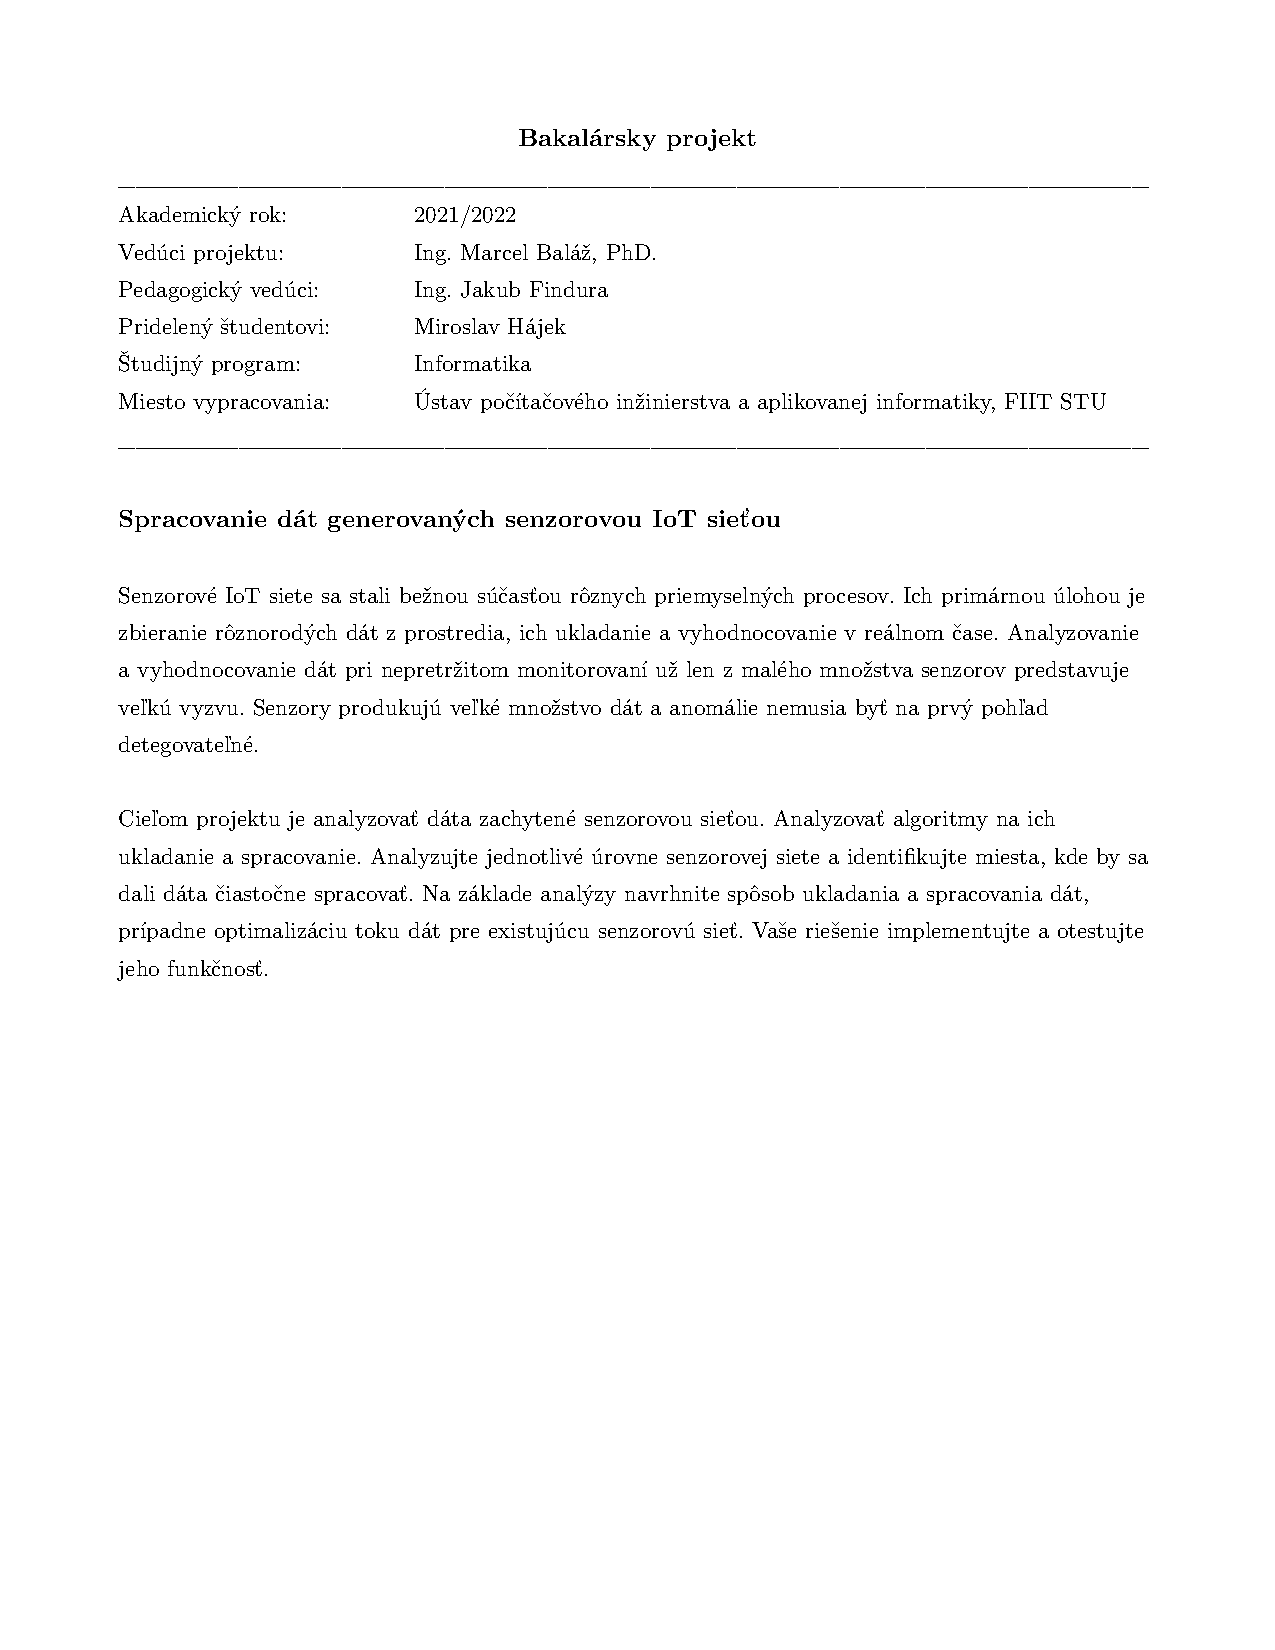
\includepdf[pages=1, scale=0.85]{zadanie}
\newpage

\emptypage
\pagenumbering{roman}

% Poďakovanie
\thispagestyle{empty}
\vspace*{\fill}
\section*{Poďakovanie}
Chcel by som sa poďakovať vedúcemu práce Ing.~Marcelovi Balážovi,~PhD. za ústretovosť, mnohé cenné pripomienky a podnety k vylepšeniam, usmernenia pri vytýčení zamerania a povzbudenie ku tvorivému preskúmaniu problematiky. 

Za poskytnutie  senzorovej jednotky a za postrehy ku formálnej stránke vďačím Ing.~Lukášovi Doubravskému. 

Tiež ďakujem svojmu kolegovi Ing.~Michalovi Juranyimu, ktorý ma za roky spolupráce mnohému priučil o vývoji softvéru.
Veľmi si cením morálnu podporu popri štúdiu od rodičov a od najbližšieho okruhu spolužiakov -- kamarátov.
\vspace{3cm}

%Anotácia
\thispagestyle{empty}
\section*{Anotácia}
\University \\
\uppercase{\Faculty}
\vspace{-8pt}
{\setlength{\mathindent}{0cm}
\begin{align*}
&\text{Študijný program:} && \text{\StudyProgramme} \\
&\text{Autor:} && \text{\Author} \\
&\text{\Thesis:} && \text{\Title} \\
&\text{Vedúci bakalárskej projektu:} && \text{\Supervisor} \\
&\text{Pedagogický vedúci:} && \text{\PedagogicalSupervisor} \\
&\text{\Date}
\end{align*}}
Stručná charakteristika zadania bakalárskeho projektu ale predovšetkým výsledkov bakalárskeho projektu v slovenskom a anglickom jazyku každá v rozsahu max. 1 strany A4 (hlavička + cca 150-200 slov).
\emptypage

%Anotácia EN
\thispagestyle{empty}
\section*{Annotation}
\UniversityEN \\
\uppercase{\FacultyEN}
\vspace{-8pt}
{\setlength{\mathindent}{0cm}
\begin{align*}
&\text{Degree course:} && \text{\StudyProgrammeEN} \\
&\text{Author:} && \text{\Author} \\
&\text{\ThesisEN:} && \text{\TitleEN} \\
&\text{Supervisor:} && \text{\SupervisorEN} \\
&\text{Departmental advisor:} && \text{\PedagogicalSupervisorEN} \\
&\text{\DateEN}
\end{align*}}
Annotation text in English, 150-200 words.
\emptypage 


% Obsah
\renewcommand{\contentsname}{Obsah}
\thispagestyle{empty}
\tableofcontents{}
\emptypage

% Kapitoly
\pagenumbering{arabic}

\chapter{Úvod}
Inteligentné senzorové systémy zariadení internetu vecí zaznamenávajú obrovskú kvantitu údajov z prostredia, kde
pôsobia. Prúdy vzoriek meraných veličín majú samy osebe nízku informačnú hodnotu. Zbytočne zaťažujú
prenosové pásmo komunikačných kanálov a kapacitu úložísk. Monitorovanie širokého rozsahu kladie požiadavky
na nízke výrobné náklady senzorových jednotiek a dlhodobú výdrž pri napájaní z batérií za minimálnej údržby.
Existuje preto potreba získané dáta spracovať do istej miery už v blízkosti ich zdroja, aby došlo k efektívnemu
využitiu dostupných prostriedkov.

Význam a dôležitosť sledovania vibrácií spočíva v ich výskyte u každého mechanického zariadenia pohybom jednotlivých súčiastok
a trením v ložiskách. Ich nadmerná prítomnosť býva spôsobená opotrebením dielov stroja alebo dôsledkom technických defektov.
Ďalšou oblasťou hojnej prítomnosti vibrácií je preprava osôb a tovaru. Tam sú zapríčinené nerovnosťami povrchu vozovky
alebo koľaje v bode styku s kolesami, či aparátom ovplyvňujúcim pohyb vozidla. Menovite ich vyvoláva točivý moment
spaľovacieho alebo elektrického motora a činnosť brzdového systému.

Detekciou nežiaducich vibrácií v preprave sa dokáže zabezpečiť bezpečnosť pasažierov včasnou výmenou súčiastky,
ktorá by ovplyvnila prevádzkyschopnosť v kritických momentoch. Ich odhalením predchádzame nenávratnému poškodeniu krehkých materiálov,
znehodnoteniu reaktívnych substancií, či ich aktivácii v prípade výbušnín a pyrotechniky. Vibrácie sú súčasťou
nebezpečných prírodných úkazov a správna identifikácia má za následok varovania na evakuáciu obyvateľstva
v oblasti postihnutej zemetrasením, či erupciou sopky, vedúcimi k ohrozenia zdravia osôb a poškodenia majetku.

Vibračný signál je merateľný v digitálnej podobe snímačom pohybového zrýchlenia mikromechanickej konštrukcie, o čom
pojednávame v kapitole \ref{chapter:analysis}. Na postupnosť pozorovaní sa nazerá ako vlnový priebeh,
ktorý sa sprehľadňuje agregačnými, korelačnými a testovacími štatistikami na odhalenie náhlych zmien.
Významne úrovne sa odlišujú od nevýznamných algoritmami na detekciu špičiek. Metódami transformácie do frekvenčnej oblasti
sa objavujú periodicky prítomné zložky. Modely spracovania majú byť nasadené do adekvátnej vrstvy senzorovej siete.
V kapitole \ref{chapter:design} popíšeme hardvér, pre ktorý navrhneme firmvér uskutočňujúci sústavu
krokov na extrakciu udalostí z vektora zrýchlenia a predstavíme dátové sady na validáciu funkčnosti.
Ďalej v kapitole \ref{chapter:implementation} je prezentovaná implementácia najdôležitejších štruktúr a komponentov. Nakoniec
riešenie overíme v kapitole \ref{chapter:verification} a dosiahnuté výsledky okomentujeme v kapitole \ref{chapter:evaluation}.




\chapter{Analýza}

\section{Monitorovanie vibrácií a šoku}
Vibrácie sú periodickým kmitaním hmoty okolo rovnovážnej polohy vznikajúce excitáciou látky, ktorej je dodaná potenciálna energia, a zo
zákona zachovania energie je následne premieňaná na kinetickú energiu. V realite dochádza pôsobením trenia k útlmu voľného oscilačného
pohybu s časom  a pohybová energia sa uvoľňuje v podobe tepelnej alebo akustickej emisie do okolitého prostredia. Častejšie ako presné
harmonické kmity sú pozorované náhodné vibrácie, ktorých vývoj nevieme dopredu predvídať. Naproti tomu šok, alebo aj prechodový jav, je
náhle uvoľnenie kinetickej energie krátkeho trvania oproti prirodzenej oscilácii systému.

Význam a dôležitosť sledovania vibrácií spočíva v ich výskyte u každého mechanického zariadenia a je zapríčinená pohybom jednotlivých
súčiastok a trením v ložiskách. Ich nadmerná prítomnosť býva spôsobená opotrebením dielov stroja alebo nevyvážením rotačných častí,
zakliesňovaním ozubených kolies, ako dôsledkoch iných technických defektov. V prevažnej väčšine prípadov ide o nežiaduci jav nakoľko
zakladá zníženiu účinnosti so zvýšením hlučnosti ako vedľajšiemu produktu.

Ďalšou oblasťou hojnej prítomnosti vibrácií je preprava osôb alebo tovaru cestnými a železničnými dopravnými prostriedkami, kde sú
zapríčinené nerovnosťami povrchu vozovky alebo koľaje v bode styku s kolesami vozidla. Na zvýšenie ovládateľnosti vozidla a komfortu
pasažierov sú kabíny odpružené od kolies tlmičmi. Lietadlá sú zasa pod vplyvom trenia vzduchu s trupom a krídlami konštrukcie, ktoré je
ďalej zosilnené vzdušnými prúdmi a turbulenciami.

Druhým významným faktorom podieľajúci sa na tvorbe vibrácii je aparát, ktorý uvádza vozidlo do pohybu alebo zastavuje, čiže hnací
najčastejšie spaľovací, dieselový alebo elektrický motor a brzdový systém. Jedná sa najmä o vplyv pohybu piestov, alebo rotora u
elektrických vozidiel, a prenosu otáčavého pohybu motora cez oje hriadeľa na nápravy. ABS brzdový systém prítomný pri väčšine
automobilov zabraňujú šmyku striedavým zomknutím a uvoľňovaním brzdových kotúčov, čo má tiež vplyv na podmienky počas jazdy.

Detekciou nežiaducich vibrácií v preprave sa dokáže zabezpečiť aj bezpečnosť pasažierov včasnou výmenou súčiastky, ktorá by ovplyvnila
prevádzkyschopnosť v kritických momentoch. Ich eliminácia dokáže predísť nenávratnému poškodeniu krehkých materiálov alebo
znehodnoteniu reaktívnych substancií, či dokonca ich aktivácii v prípade výbušnín a pyrotechniky.

V neposlednom rade sú vibrácie súčasťou potenciálne nebezpečných prírodných úkazov a ich správna identifikácia má za následok varovania
pre preventívnu evakuáciu obyvateľstva v oblasti, ktoré bude zasiahnutá zemetrasením, či erupciou sopky vedúcimi k ohrozenia zdravia
osôb a poškodenia majetku.

\subsection{Meranie fyzikálnej veličiny akcelerácie}
Pohyb mechanického systému vystaveného vonkajším silám sa nazýva odozva, ktorej správanie opisuje zjednodušený model s jedným stupňom
voľnosti (1DOF) kmitajúceho telesa s pružinou a tlmičom \cite{vibrations-shock}.

\begin{figure}[h]
	\centering
	
\includegraphics[width=0.7\textwidth]{figures/mass-spring-damper-model.png}
	\caption{Model oscilujúceho systému s pružinou a tlmičom}
\end{figure}

Pri pôsobení vonkajšej sily $F$ na hmotu upevnenú na pružine vznikajú nútené vibrácie, ktoré ju vychyľujú z rovnovážnej polohy.
Uvedená sila je charakterizovaná druhým Newtonovým zákonom v tvare $F = ma$, kde $m$ je hmotnosť telesa a $a$ predstavuje zrýchlenie.
V protismere pôsobí sila vyvolaná pružinou $F_s = -kx$ a tlmiacim členom $F_d = -cv$, kde $k$ je tuhosť pružiny ovplynená jej konštrukciou,
$c$ je tlmiaci koeficient, $x$ je vychýlenie z rovnovážneho stavu, a $v$ rýchlosť vychýlenia.

Fyzickým obmedzením  telesa, ktorým je viazaný na pevnú podložku dochádza pri zanedbaní deformácie k takmer zaručenému návratu do rovnovážnej
polohy a to nám umožňuje merať intenzitu vibrácií cez zrýchlenie ťažidla. Výslednú silu v jednom smere získame sčítaním síl podieľajúcich sa na dynamike telesa.
\myequations{Fyzikálny model oscilujúceho systému s pružinou a tlmičom}
\begin{ceqn}\begin{align}
 	F(t) = ma - cv - kx
\end{align}\end{ceqn}

Pri použití trojosového akcelerometra, kedy sú evidované všetky tri priestorové súradnice časovo-premennej akcelerácie dostávame
nasledujúcu rovnicu vo vektorovom tvare:
\myequations{Newtonov zákon sily}
\begin{ceqn}\begin{align}
   \vec{a}(t) = \frac{\vec{F}(t)}{m}
\end{align}\end{ceqn}

Magnitúda akcelerácie s troma súradnicami je daná $L_2$ normou vektora $\vec{a} = (a_x, a_y, a_z)$:
\myequations{Magnitúda vektora akcelerácie}
\begin{ceqn}\begin{align}
   |a| = \sqrt{a_x^2 + a_y^2 + a_z^2}
\end{align}\end{ceqn}

\subsection{MEMS kapacitný akcelerometer}
Bežné inerciálne senzory na meranie zrýchlenia priamočiareho, ale aj rotačného pohybu (gyroskop), sa vyrábajú technológiou
\emph{MEMS – mikromechanický systém}, kedy je celé zariadenie vrátane všetkých mechanických súčastí umiestnené na kremík procesom
mikrovýroby vo viacerých vrstvách. Sila spôsobujúca zrýchlenie je potom meraná vychýlením vstavanej odpruženej hmoty vzhľadom
na pevné elektródy, ktoré môžu byť usporiadané jednostranne alebo ako diferenčný pár \cite{mdof-mems-accelerometers}.

\begin{figure}[h]
	\centering
	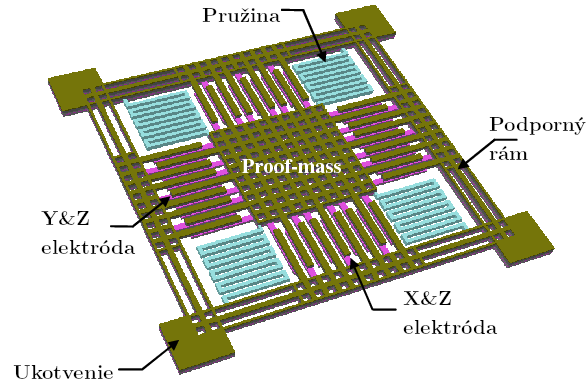
\includegraphics[width=0.8\textwidth]{figures/mems-accelerometer.png}
	\caption{Mikroštruktúra 3DOF MEMS kapacitného akcelerometra \cite{microstructure-mems}}
	\label{fig:mems}
\end{figure}

Pri diferenčnom páre spôsobí pohyb doštičky ťažidla medzi elektródami zmenu kapacít a ich rozdielom je možné zistiť aplikovanú silu a
cez uvedený vzťah zrýchlenie. Na zvýšenie celkovej kapacity sa používa viacero párov elektród zapojených paralelne. Pred prevodom na
číslicový signál musí napäťová úroveň zo senzora prejsť úpravou zahŕňajúcou nábojovocitlivý predzosilňovač, osovú demoduláciu a anti-
aliasingové filtrovanie.

Viacosové akcelerometre vyžadujú viaceré opísané štruktúry orientované kolmo na seba, podľa obr. \ref{fig:mems}, s ohľadom na počet
vyžadovaných stupňov voľnosti, pričom v skutočných senzoroch vždy existuje aspoň minimálna závislosť medzi osami rádovo najviac v
jednotkách percent. Teplota ovplyvňuje citlivosť MEMS akcelerometrov len nepatrne v stotinách percenta na stupeň Celzia.

Akcelerometre sa odlišujú v niekoľkých dôležitých vlastnostiach, ktoré zvyknú byť nastaviteľné vo výrobcom stanovenom rozsahu
prípustných hodnôt s príslušnými toleranciami \cite{accelerometer-mechanics}.

\emph{Citlivosť} stanovuje najmenšiu rozlíšiteľnú zmenu v odčítanom napätí ku zmene externého pohybu respektíve zrýchlenia.
Uvádza sa v jednotkách \emph{mV/g} (milivolt na tiažové zrýchlenie) pri analógovom výstupe, alebo \emph{mg/LSB} (mili-g
na najmenej významový bit). pri senzoroch so vstavaným analógovo-digitálnym prevodníkom. Jednotka \emph{mg/LSB} vyjadruje
o koľko sa zmení zrýchlenie keď zvýšime alebo ponížime binárne číslo na výstupe o jedna. Niekedy sa namiesto
citlivosti uvádza mierka pre presnosť ako prevrátená hodnota citlivosti v \emph{LSB/g}. Tiažové zrýchlenie $g$ sa mierne líši podľa
zemepisnej šírke, ale stanovený prepočet na jednotky SI je $1 g = 9.80665\,m/s^2$
\footnote{\url{https://physics.nist.gov/cgi-bin/cuu/Value?gn|search_for=acceleration}}.

\emph{Dynamický rozsah} sa uvádza v tiažovom  zrýchlení $g$. Hovorí o najmenšej a najväčšej rozlíšiteľnej hodnote zrýchlenia nad
úrovňou ktorej už dochádza k skresleniu signálu orezaním špičiek. S nevyhnutnými drobnými nepresnosťami výroby mikromechaniky je tzv.
\emph{zero-g napätie} popisujúce odchýlku skutočného od ideálneho výstupu, keď na sústavu nepôsobí žiadne zrýchlenie. Za ideálnych
okolností bez pohybu na vodorovnom povrchu namerajú osi $x$ a $y$ zrýchlenie $0g$, zatiaľčo na $z$ pôsobí $1g$. Očakávaním je nulová
hodnota výstupného napätia a tým aj výstupného registra.

\emph{Šírka pásma} senzora v \emph{Hz} predurčuje rozsah frekvencie vibrácií, ktoré je možné zachytiť. Podmienená je zvolenou
početnosťou  čítania akcelerácie za sekundu, čiže vzorkovacou frekvenciou. Stanovuje sa tiež nastaviteľným parameterom \emph{ODR}
(Output Data Rate) - výstupný dátový tok, pričom šírka pásma je spravidla polovicou ODR. Menej uvádzanou vlastnosťou býva
\emph{frekvenčná odozva} senzora, ktorá určuje o koľko sa v rámci tolerancie odlišuje skutočná
citlivosť od referenčnej pre zodpovedajúcu frekvenciu vibrácii.

Na meranie zrýchlenia má nevyhnutný vplyv šum zapríčinený Brownovým  pohybom a nedokonalosťou skutočných materiálov v štruktúre
akcelerometra. Intenzita šumu rastie inverznou odmocninou so šírkou pásma, čiže s častejším meraním získavame menšiu presnosť. Pri
dostatočnom odstupe signálu od šumu, $SNR = P_{signal} / P_{šum}$, umožňuje hardvér akcelerometra vzorkovať amplitúdy až nad stanovený
prah generovaním prerušenia, čím sa dokáže efektívne zbaviť nevýznamných fluktuácií.

\subsection{Analógovo-digitálny prevodník}
Spojitá napäťová úroveň transformuje analógovo-digitálny (A/D) prevodník pre spracovanie digitálnym systémom do množiny diskrétnych
hodnôt. Vstupný signál najprv prechádza fázou vzorkovania, kedy sa vzorky zaznamenávajú v pravidelných intervaloch. Počet vzoriek
odčítaných za sekundu je vyjadrený vzorkovacou frekvenciou $f_s$ v $Hz$. Časový rozdiel medzi vzorkami, nazývaný perióda vzorkovania,
je prevrátenou hodnotou vzorkovacej frekvencie $T_s = \frac{1}{f_s}$. Pre presnú rekonštrukciu pásmovo obmedzeného signálu v hraniciach
$[-f_{max}; f_{max}]$ je nevyhnuté podľa \emph{Nyquist-Shannonovej vety} o vzorkovaní, aby vzorkovacia frekvencia bola najmenej
dvojnásobkom maximálnej frekvencie snímaného signálu.
\myequations{Nyquist-Shannonova veta o vzorkovaní}
\begin{ceqn}\begin{align}
   f_s \geq 2 \cdot f_{max}
\end{align}\end{ceqn}

V procese kvantovania je každej vzorke je následnepriradená diskrétna hodnota s konečným počtom $n$ bitov, ktorá je najbližšia
možná ku skutočnej hladine analógového vstupu. Dochádza pritom k istému zaokrúhľovaniu z dôvodu nepresnosti vyjadrenia spojitej
domény amplitúd diskrétnym číslom. Tento jav označujeme ako kvantizačný šum, ktorý je najviac polovicou z maximálnej rozlíšiteľnej
zmeny signálu a trpia nim všetky existujúce A/D prevodníky.

\begin{figure}[h]
	\centering
	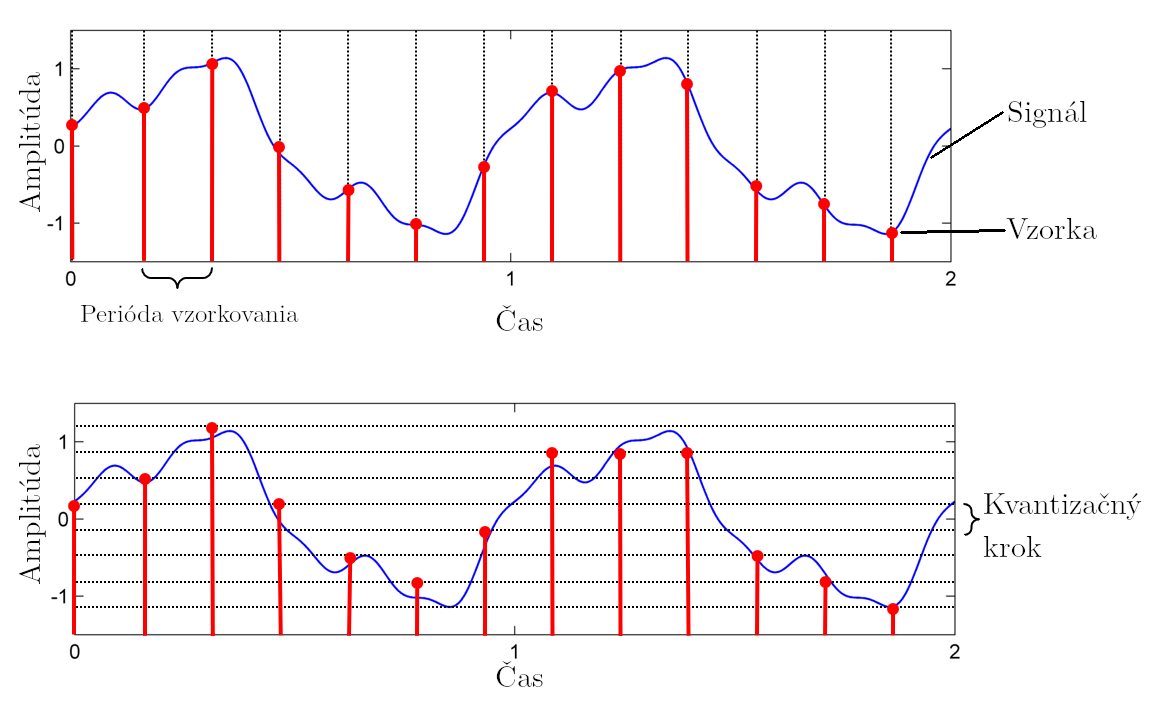
\includegraphics[width=0.8\textwidth]{figures/analog-to-digital-conversion.png}
	\caption{Digitalizácia signálu v analógovo-digitálnom prevodníku \cite{music-processing}}
\end{figure}

Prevodníky integrované priamo s inerciálnymi jednotkami sa vyhotovujú v rozlíšeniach 12, 16 alebo 20 bitov. Umožňujú tak pripojiť
akcelerometer rovno na sérové zbernice \emph{SPI} alebo \emph{I2C}. Všeobecne platí, že pri $n$ bitoch je k dispozícii $2^n$ rozličných
čísel. Kódovaním v dvojkovom doplnku pre zachytenie záporných hodnôt sa uvažuje s intervalom $[-2^\frac{n}{2}; 2^\frac{n}{2} - 1]$.

Číslicová hodnota v dvojkovom doplnku získanú konverziou $\hat{x}$ je prepočítaná na
štandardné fyzikálne jednotky pre zrýchlenie, $a$ v $m/s^2$). $R$ prestavuje nastavený dynamický rozsah v jednotkách $g$ a $n$
je počet bitov A/D prevodníka.
\myequations{Konverzia merania na akceleráciu podľa rozlíšenia A/D prevodníka}
\begin{ceqn}\begin{align}
   a = \hat{x} \cdot ((R \cdot g) / 2^{n / 2})
\end{align}\end{ceqn}

Na základe už zmieneného ohľadom vlastností MEMS akcelerometrov, presnejší prevod dosiahneme zužitkovaním deklarovanej citlivosti
senzora pri danom dynamickom rozsahu $S_R$ udávaného v $mg/LSB$.
\myequations{Prevod A/D prevodníkom u akcelerometra s rozsahom v $mg/LSB$}
\begin{ceqn}\begin{align}
   a = \hat{x} \cdot (S_R \cdot g) / 1000
\end{align}\end{ceqn}

\subsection{Vlastnosti bežných akcelerometrov}
Na ilustráciu uvádzame parametre zvolených najrozšírenejších typov akcelerometrov. Akcelerometer LSM9DS1 \cite{lsm9ds1} umožňuje cez
zbernicu SPI alebo I2C zvoliť zo štyroch dynamických rozsahov, pričom každé rozpätie sa vyznačuje svojou citlivosťou. Zvolením menšieho
dynamického rozsahu zvýšime citlivosť. LSM9DS1 funguje pri rozsahoch $\pm2$g, $\pm4$g a $\pm8$g a $\pm16$g, postupne s citlivosťami
$0.061$ mg/LSB, $0.122$ mg/LSB, $0.244$ mg/LSB, $0.732$ mg/LSB. Výstupný dátový tok (ODR) je možné nastaviť na $10$Hz, $50$Hz,
$119$Hz, $238$Hz, $476$Hz a najvyššie na $952$ Hz. Navzorkované hodnoty sú ukladané do 16-bitového výstupného registra v
dvojkovom doplnku.

Nízkoenergetický 3DOF MEMS akcelerometer ADXL362 \cite{adxl362} so spotrebou $2\,\mu A$ pri $100$Hz disponuje
rozsahmi $\pm2$g, $\pm4$g a $\pm8$g s citlivosťami $1$, $2$ a $4$ mg/LSB. Dostupné vzorkovacie frekvencie 12-bitového A/D prevodníka sú
$12.5 - 400$Hz v 8 krokoch vždy po násobkoch predošlého kroku. Pre rýchlejšie čítanie pri nižšom rozlíšení dokáže senzor zakódovať dáta
do 8-bitového registra.

Vyrábajú sa tiež akcelerometre s väčšími dynamickými rozsahmi a nízkym šumom, ide napríklad o ADXL356 a ADXL357 \cite{adxl357} so
škálami $\pm 10$g, $\pm 20$g a $\pm 40$g s citlivosťou $0,019$ mg/LSB po $0,078$ mg/LSB a rozlíšením A/D prevodníka 20 bitov pri
ODR $4 - 4000$Hz. ADXL357 ponúka priamo analógové výstupy s citlivosťou $20 - 80$ mV/g pri napájaní $3.3$ V.

\subsection{Odvodzovanie rýchlosti a dráhy zo zrýchlenia}
Meranie akcelerácie umožňuje zároveň nepriamo získať ďalšie údaje o pohybe celkovom v priestore ako aj spôsobenom vibráciami.
Zrýchlenie $\vec{a}$ je definované ako časová zmena rýchlosti $\vec{v}$, zatiaľčo rýchlosť je časovou zmenou polohy $\vec{r}$. Na
pozorovanie prechodových javov alebo na vyjadrenie miery plynulosti pohybu slúži ryv $\vec{j}$, ktorý je časovou zmenou akcelerácie.
Pokiaľ nie sú známe počiatočné podmienky v okamihu začiatku snímania akcelerácie, budú hodnoty veličín relatívne vzhľadom na
štart záznamu. Kinematika v diskrétnom čase je potom opísaná nasledujúci rovnicami, kde $\Delta$ je operátor diferencie
$\Delta t = t(i) - t(i-1)$:
\myequations{Kinematické rovnice pre polohu, rýchlosť, zrýchlenie a ryv}
\begin{ceqn}\begin{align}
   \vec{v} = \frac{\Delta \vec{r}}{\Delta t}; \;\;
   \vec{a} = \frac{\Delta \vec{v}}{\Delta t}; \;\;
   \vec{j} = \frac{\Delta \vec{a}}{\Delta t}
\end{align}\end{ceqn}

Vyjadrenie neznámych premenných vzhľadom na akceleráciu spočíva v prenásobení rovníc členom $\Delta t$, čím sa získajú
vzťahy pre okamžitú dráhu a okamžitú rýchlosť. Spočítaním čiastkových okamžitých rýchlostí na intervale dostaneme celkovú rýchlosť a
rovnaký úsudok platí pre polohu. V spojitom čase, keď by vzorkovacia perióda bola nekonečne krátka, dochádza naproti tomu k
integrovaniu funkcie akcelerácie. Dostávame, že rýchlosť je integrálom zrýchlenia a poloha je dvojným integrálom zrýchlenia:
\myequations{Rýchlosť a poloha cez integrál akcelerácie}
\begin{ceqn}\begin{align}
   \vec{v}(t) = \vec{a_0} + \int{\vec{a}(t)\,\mathrm{dt}} \\
   \vec{r}(t) = \vec{r_0} + \vec{v_0}t + \iint{\vec{a}(t)\,\mathrm{dt}}
\end{align}\end{ceqn}


\subsection{Numerická kvadratúra}
Približný výpočet určitého integrálu funkcie akcelerácie je založený na geometrickej interpretácii integrálu ako plochy pod krivkou.
Hovoríme vtedy o probléme numerickej kvadratúry, ktorý navrhuje nahradiť pôvodný integrand interpolačným polynómom
\cite{numerical-mathematics}. Rád polynómu $n$ implicitne stanoví priebeh funkcie medzi ekvidištantnými vzorkami a
má dopad na presnosť aproximácie. Najčastejšie sa používajú konštantný ($n = 0$), lineárny ($n = 1$) alebo kvadratický ($n = 2$)
polynóm, podľa toho rozlišujeme obdĺžnikové pravidlo (vzorec \ref{eq:midpoint-rule}),
lichobežníkové pravidlo (vzorec \ref{eq:trapezodial-rule}) a Simpsonovo pravidlo (vzorec \ref{eq:simpson-rule}).
\myequations{Pravidlá numerickej kvadratúry: obdĺžníkové, lichobežníkové, Simpsonovo}
\begin{ceqn}
\begin{align}
   v(t_i) &= T_s \cdot a\left(\frac{t_i + t_{i-1}}{2}\right)  \label{eq:midpoint-rule} \\
   v(t_i) &= \frac{T_s}{2} \cdot [a(t_i) + a(t_{i-1})]		\label{eq:trapezodial-rule} \\
   v(t_i) &= \frac{T_s}{3} \cdot [a(t_{2i}) + 4a(t_{2i - 1}) + a(t_{2i - 2})] \label{eq:simpson-rule}
\end{align}
\end{ceqn}

Pri \emph{obdĺžníkovom pravidle} (obr. \ref{fig:midpoint-rule}) nepripúšťame zmenu hodnoty zrýchlenia medzi vzorkami a okamžitú
rýchlosť, čiže plochu, odhadneme ako dĺžku intervalu vzorkovania vynásobenú priemerom výšok dvoch následných pozorovaní. Interpolačný
polynóm je konštantná funkcia. \emph{Lichobežníkové pravidlo} (obr. \ref{fig:trapezodial-rule}) uvažuje s lineárnou zmenou veličiny
medzi meraniami, preto interpoluje priamkou.\emph{Simpsonovo pravidlo} (obr. \ref{fig:simpson-rule}) sa snaží o ešte tesnejší odhad s
využitím kvadratickej funkcie. Každé kvadratúrne pravidlo sa síce vyznačuje presne vyčísliteľnou chybovosťou, ale k tomu je nevyhnutné
poznať analytické vyjadrenie vibrácií, čo dáva realistický odhad len pri čisto periodických kmitoch.

\begin{figure}[h]
\centering
\begin{subfigure}[b]{0.32\textwidth}
    \centering
    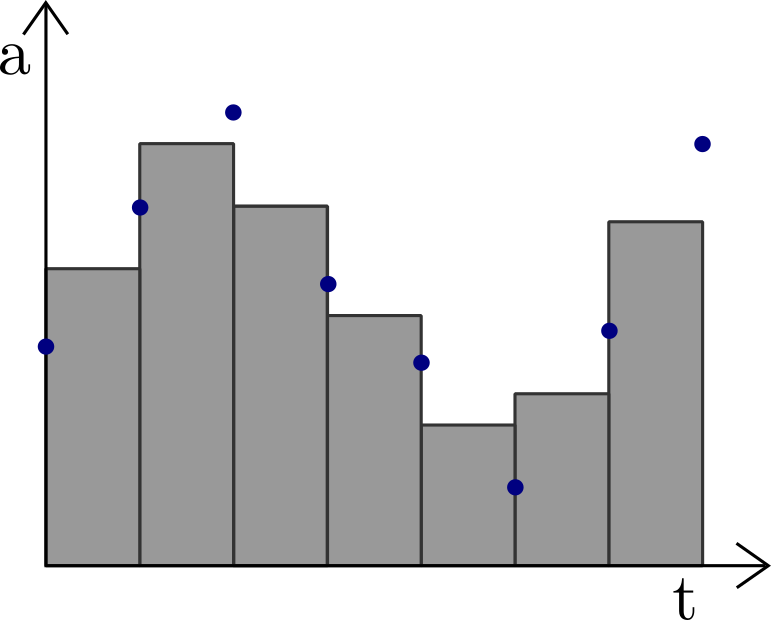
\includegraphics[width=\textwidth]{figures/rectangular-rule.png}
    \caption{Obdĺžníkové}
    \label{fig:midpoint-rule}
\end{subfigure}
\hfill
\begin{subfigure}[b]{0.32\textwidth}
    \centering
    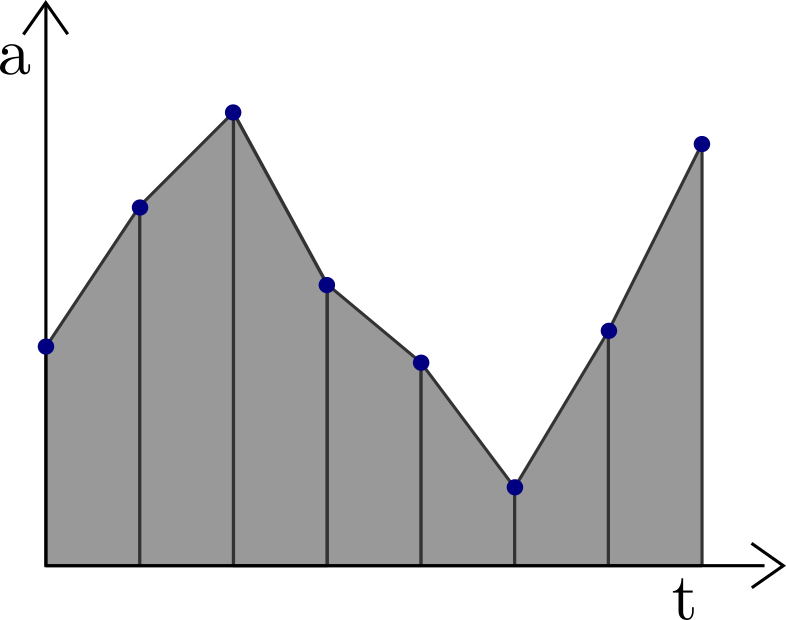
\includegraphics[width=\textwidth]{figures/trapezoidal-rule.png}
    \caption{Lichobežníkové}
    \label{fig:trapezodial-rule}
\end{subfigure}
\hfill
\begin{subfigure}[b]{0.32\textwidth}
    \centering
    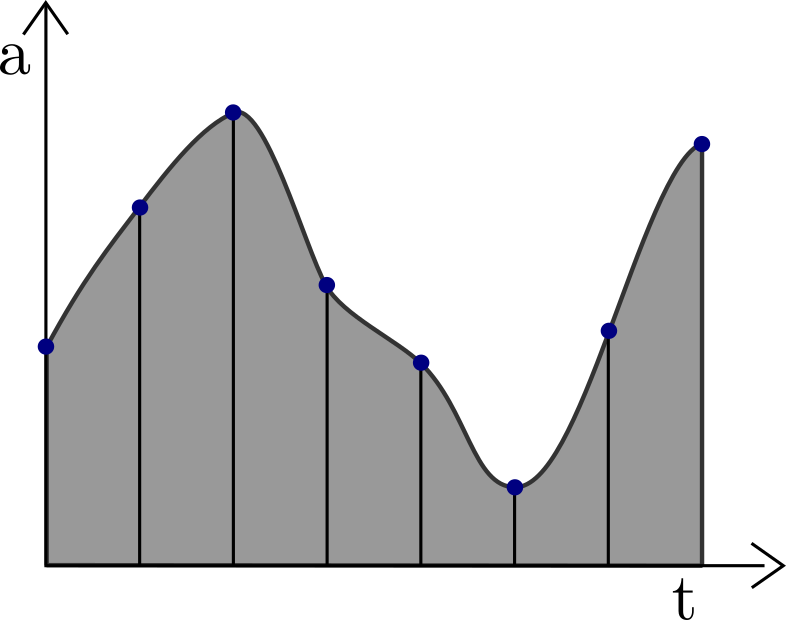
\includegraphics[width=\textwidth]{figures/simpson-rule.png}
    \caption{Simpsonovo}
    \label{fig:simpson-rule}
\end{subfigure}
\caption{Porovnanie pravidiel numerickej integrácie}
\end{figure}

Priama integrácia zašumeného signálu zrýchlenia vedie k neskutočnému driftu, ktorý je ešte zvýraznený dvojitou integráciou pri
odvodzovaní relatívneho posunutia. Dochádza k zosilneniu nízkych a potlačeniu vyšších frekvencií, čím sa začne dominovať neexistujúci
trend vo výstupných dátach. Očakávané oscilujúce správanie vychýlenia u vibrácií so zväčšujúcim sa počtom sčítancov pri rekurentnom
výpočte zaniká. Na zlepšenie stability integrátora sa uplatňuje korekcia cez obálky \cite{integration-acceleration-envelopes}.

Najprv je na vstupnom signále vykonaná zvoleným pravidlom numerická kvadratúra, ktorá môže byť realizovaná na krátkych
úsekoch funkcie, aby sa predišlo pretečeniu pri výraznej akumulácií odklonu. Prichádza k identifikácií lokálnych extrémov a ich interpoláciou s kubickou B-spline sa sformuje horná $e_u(t)$, respektíve dolná
obálka signálu $e_d(t)$. Obálky sú spriemerované $\bar{e}(t)$ za vzniku odhadu trendovej krivky, ktorá je od už integrovaného
signálu odčítaná $g(t) = f(t) - \bar{e}(t)$. V prípade výpočtu polohy je možné aplikovať uvedený postup kaskádovito, čiže rovnako
ako akcelerácia je aj signál rýchlosti opäť integrovaný a korigovaný obálkami.

\section{Metódy analýzy signálu v časovej doméne}
Pozorovania veličiny predstavujú udalosti merané sekvenčne v čase, kde je s každou obdržanou hodnotou $x_i$ viazaná unikátna
časová značka $t_i$. Postupnosť jednotlivých čítaní je jednorozmerný časový rad znázoriteľný ako usporiadaná množina dvojíc pečiatky
rastúcej v čase a nasnímanej úrovne: $T = \{(t_1, x_1),(t_2, x_2), …, (t_n, x_n)\}$. Vzorkovaním v pravidelných intervaloch stačí
uvažovať namiesto časových značiek o celočíselných indexoch, ktoré určujú pozíciu prvkov vo vektore pozorovaní:
$\mathbf{x} = (x_1, x_2, …, x_n)^T$.

\subsection{Prúdové algoritmy}
Pri veľkom objeme prichádzajúcich vzoriek produkované senzormi, nie je uskutočniteľné ich úplné uchovanie ani spracovanie celkého
dátového toku naraz. Častokrát by stratégia neuváženého odkladania viedla k plýtvaniu zdrojov a zbytočnému archivovaniu údajov s nízkou
informačnou hodnotou. Vhodnejšie je agregovanie toku údajov podľa preddefinovaného zmysluplného kritéria, ktoré zachytáva
významné rysy a prompte zodpovedať na vyžadované dopyty.

Priamočiarou realizáciou agregácie je nahliadať na prvky časového radu postupne ako prichádzajú.
Prúdové algoritmy pôsobiace v reálnom čase, a teda neschopné vidieť finálny vektor vzoriek vstupu sa vyznačujú vlastnosťou, že
vyprodukujú len na základe takého čiastkového vstupu parciálny výsledok platný pre dosiaľ sa vyskytnutú podmnožinu.

Za ideálnych okolností by sa mal online algoritmus učiť kontinuálne bez ukladania predošlých bodov a detekcií.
V rozhodnutiach algoritmu sú zahrnuté informácie o všetkých predošlých bodoch do terajšieho rozhodnutia.
Mal by mať schopnosť sa adaptovať dynamickému prostrediu, v ktorom pôsobí, bez nutnosti manuálnych úprav parametrov modelu.
Zároveň je žiaduce minimalizovať falošné pozitíva a negatíva pri detekcii udalostí. \cite{data-streams}.

\subsection{Posuvné a rozširujúce sa okná}
Časový rad $\left(x_i\right)_{i = 0}^{n}$ s dĺžkou $n$ môže byť pre účely výpočtu sumárnych štatistík rozdelený oknovou funkciou
$\mathcal{W}_{l, d}$ na podpostupnosti nazývané okná.

\emph{Posuvné okná} (,,rolling window'') majú spravidla konštatnú dĺžku $l$
menšiu ako celkovú veľkosť radu a sú aplikované s krokom odstupu $d$ pozorovaní. Rad pozorovaní pozostáva z $ (n - (l  - 1)) / d$
okien \cite{online-anomaly-detection}. Prirodzene sa posuvné okná objavujú pri manipulácii s vyrovnávacou pamäťou, ktoré sa využívajú
pri blokovom prenose z adaptéra senzora do hlavnej pamäte. Vtedy sa veľkosť bloku sa rovná posunu $l = d$.

\emph{Rozširujúce sa okná} (,,expanding window'') nachádzajú uplatnenie v menej prípadoch, spravidla sa jedná o inkrementálny
odhad globálnej štatistiky, ktorá má zmysel prevažne pri sledovaní stabilného javu. \cite{practical-time-series}. Okno začína na
stanovenej minimálnej veľkosti a s pribúdajúcim počtom bodov ich zahŕňa, čím sa zväčšuje.

\subsection{Číselné charakteristiky štatistického rozdelenia}
Náhodné vibrácie vyskytujúce sa pri skutočných materiáloch sú stochastický proces, ktorý tvorí sekvencia časovo indexovaných
náhodných premenných. Časový rad predstavuje realizáciu tohto stochastického procesu $\mathbf{Y} = (X_1, X_2, ..., X_n)^T$, kde $X_t$
je náhodná premenná so svojím rozdelením pravdepodobnosti. Všeobecne sa pri ideálnych stacionárnych otrasoch predpokladá, že premenné
pochádzajú z unimodálnej Gaussovej distribúcie: $X_t \sim N(\mu, \sigma^2)$ \cite{vibrations-shock}.

Sumárna deskripcia nameraného deja pre extrakciu typických čŕt konkrétnych pozorovaných situácií sa uskutočňuje viacerými štatistikami
$h(X_1, X_2, ..., X_n)$ zostručňujúcimi opis funkcie hustoty rozdelenie. Na rozmiestnenie hodnôt meraní v priebehu časového úseku
sa nazerá z pohľadu polohy, rozptýlenosti a tvaru. Rozsah oboru hodnôt je amplitúda špička-špička (,,peak-to-peak''),
ktorá je rozdielom maximálnej a minimálnej úrovne, údaj známy tiež ako variančné rozpätie \cite{zaklady-statistiky}.
\myequations{Amplitúda špička-špička}
\begin{ceqn}\begin{align}
x_{pp} = \max_{t \in \mathcal{W}}\{x_t\} - \min_{t \in \mathcal{W}}\{x_t\}
\end{align}\end{ceqn}

Priemernú energiu obsiahnutú v signále predstavuje štvorec efektívnej amplitúdy RMS a určí sa ako kvadratický priemer pozorovaní:
\myequations{Efektívna amplitúda RMS}
\begin{ceqn}\begin{align}
x_{rms} = \sqrt{\frac{1}{n}\sum_{t=1}^{n}{x_t^2}}
\end{align}\end{ceqn}

Mierami polohy rozdelenia pozorovaní sú stredná hodnota, informujúca
o centre hodnôt veličiny, a kvantily rozkladajúce usporiadaný vektor pozorovaní na určený počet rovnakých skupín.
Nevychýleným bodovým odhadom strednej hodnoty je \emph{výberový priemer}, ktorý je zároveň amplitúdou jednosmernej zložky signálu:
\myequations{Výberový priemer alebo amplitúda jednosmernej zložky}
\begin{ceqn}\begin{align}
\bar{x} = \frac{1}{n} \sum_{t = 1}^{n}{x_t}
\end{align}\end{ceqn}

Najvýznamnejším kvantilmi sú kvartily $Q_q$ vytvárajúce štyri rovnako veľké časti z pôvodných dát, konkrétne dolný kvartil $Q_1$
oddelí  25\% najmenších údajov, medián $Q_2$ predelí zoradené údaje na polovicu a horný kvartil $Q_3$ zahrnie 75\% nižších hodnôt.
Hľadaný kvartil je $k$-ty najmenší prvok v utriedenom zozname meraní, pričom podľa želaného kvartilu $q$ a počtu pozorovaní je
$k = \lceil n \cdot (1 / q) \rceil$.

Zistenie $k$-teho najmenšieho prvku s časovou zložitosťou $\mathcal{O}(n \log n)$ umožňuje ľubovoľný lepší triediaci algoritmus
napríklad triedenie zlučovaním (merge sort). Algoritmus \emph{Quickselect} dokáže taký prvok objaviť v čase $\mathcal{O}(n)$.
V každom kroku vyberie náhodný deliaci bod (pivot) a preskupí k sebe hodnoty menšie ako pivot naľavo a väčšie ako pivot
napravo. Najmenší prvok následne hľadá v časti, kde zostalo viac ako $k$ prvkov. Pokiaľ došlo k deleniu zoznamu, že pivot
zaujme presne $k$-tu pozíciu prehľadávanie je ukončené a pivot prehlásený za riešenie. Nesprávnym výberom pivota môže
v najhoršom prípade dôjsť až k zložitosti $\mathcal{O}(n^2)$, čomu sa predchádza výberom pivota cez medián mediánov.

Sústreďovanie realizácie veličiny, respektíve jej rozptýlenosť okolo strednej hodnoty vieme opísať viacerými štatistikami
ako sú \emph{výberový rozptyl} (\ref{eq:variance}), ktorej odmocninou dostaneme smerodajnú odchýlku,
\emph{priemerná absolútna odchýlka} (\ref{eq:aad}), \emph{mediánová absolútna odchýlka} (\ref{eq:mad})
a \emph{medzikvartilové rozpätie} (\ref{eq:iqr}) \cite{zaklady-statistiky}. Priemerná absolútna odchýlka je
upraviteľné o mieru centrálnej tendencie, ktorou okrem priemeru môže byť aj medián alebo modus. Vyvarovanie sa
príliš extrémnym a vychýlením hodnotám docielime zapojením práve mediánu do štatistík absolútnej odchýlky, rovnako
tak to dosiahneme medzikvartilovým rozpätím obmedzením sa na 50\% centrálnych dát.
\myequations{Výberové miery rozptýlenosti: rozptyl, smerodajná odchýlka, MAD, IQR}
\begin{ceqn}\begin{align}
	s^2 &= \frac{1}{n - 1} \sum_{t = 1}^{n}{(x_t - \bar{x})^2} \label{eq:variance} \\
	d &= \frac{1}{n} \sum_{t = 1}^{n}(|x_t - \bar{x}|) \label{eq:aad} \\
	\mathrm{MAD} &= med(|x_t - med(\mathbf{x})|) \label{eq:mad} \\
	IQR &= Q_3 - Q_1 \label{eq:iqr}
\end{align}\end{ceqn}

Numericky stabilné bežiace štatistiky priemeru a smerodajnej odchýlky sa udržiavajú cez rekurentné rovnice
\emph{Welfordovho algoritmu} \cite{knuth}. $M_1$ je aktuálna priemerná hodnota údajov v toku a $S_1$ je počítadlo pre
rozptyl, z ktorého je v ktoromkoľvek okamihu získateľná smerodajná odchýlka súboru $\sigma$:
\myequations{Welfordov algoritmus na výpočet výberového rozptylu}
\begin{ceqn}\begin{align}
   M_1 &= x_1;\quad M_k = M_{k-1} + \frac{(x_n - M_{k-1})}{k} \\
   S_1 &= 0; \quad S_k = S_{k-1} + (x_k + M_{k-1})(x_k + M_k)  \\
   \sigma &= \sqrt{S_n / (n - 1)}
\end{align}\end{ceqn}

Tvar distribúcie náhodnej premennej opisujú centrálne momenty šikmosť a špicatosť. Šikmosť $\gamma_1 = \mu^3 / \sigma^3$ udáva skosenie
rozdelenia, pričom platí že záporná šikmosť značí dlhší ľavý chvost a modus funkcie hustoty sa prevažuje napravo. Zatiaľ čo u kladnej
šikmosti je to naopak (obr. \ref{fig:skewness}).

Špicatosť $\gamma_2 = \mu^4 / \sigma^4 - 3$ (obr. \ref{fig:kurtosis}) porovnáva rozdelenie pozorovaní so strmosťou krivky normálneho rozdelenia,
čiže viacej realizácií leží bližšie alebo ďalej od strednej hodnosti. Kladná špicatosť signalizuje strmejšiu
a záporná zasa sploštenejšiu distribúciu. Platí, že $\mu_n $ je priemerom hodnôt $(x_t - \bar{x})^n$.
\begin{figure}[h]
\centering
\begin{subfigure}[b]{0.48\textwidth}
    \centering
    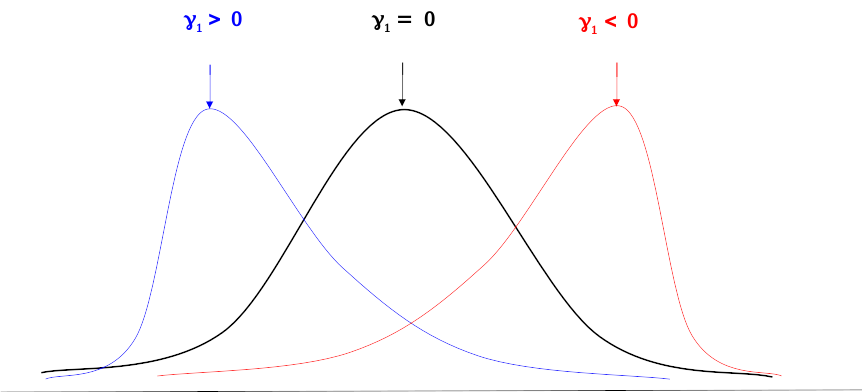
\includegraphics[width=\textwidth]{figures/skewness.png}
    \caption{Šikmosť}
    \label{fig:skewness}
\end{subfigure}
\hfill
\begin{subfigure}[b]{0.48\textwidth}
    \centering
    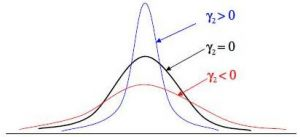
\includegraphics[width=\textwidth]{figures/kurtosis.png}
    \caption{Špicatosť}
    \label{fig:kurtosis}
\end{subfigure}
\caption{Dopad šikmosti a špicatosti na histogram distribúcie}
\end{figure}

Závislosť dvojíc veličín sa vyjadruje \emph{kovariancia} $cov(\mathbf{x}, \mathbf{y})$ a \emph{korelácia}
$\rho(\mathbf{x}, \mathbf{y})$. U vektora akcelerácie nás bude napríklad zaujímať vzájomná korelácia medzi
osami pohybu: $\rho(\vec{x},\vec{y}),\, \rho(\vec{x},\vec{z}),\, \rho(\vec{y},\vec{z})$ upozorňujúca na diagonálny
pohyb alebo podobné budenie v oboch korelovaných smeroch a tým umožňujúce redukciu údajov z dôvodu redundancie.
Kovariancia je daná strednou hodnotou súčinu odchýlky od priemeru zodpovedajúcej premennej (vzťah \ref{eq:covariance}).
Normovaním kovariancie smerodajnými odchýlkami veličín získame \emph{Pearsonov korelačný koeficient}
(vzťah \ref{eq:correlation}), ktorý je z intervalu $[-1; 1]$.  Hodnota koeficientu $-1$ značí nepriamu lineárnu závislosť
a $+1$ priamu závislosť.
\myequations{Závislosť dvoch veličín cez kovarianciu a koreláciu}
\begin{ceqn}\begin{align}
\mathrm{cov}(\mathbf{x}, \mathbf{y}) &= \frac{1}{n} \sum_{t=1}^{n}{(x_t - \bar{x})(y_t - \bar{y})} \label{eq:covariance} \\
\rho(\mathbf{x}, \mathbf{y}) &= \frac{\mathrm{cov}(\mathbf{x}, \mathbf{y})}{\sigma_x \sigma_y} \label{eq:correlation}
\end{align}\end{ceqn}

\subsection{Algoritmy na rozpoznávanie špičiek}
\label{peak-detection}
Detekcia udalostí a významných zmien signálového priebehu sa spolieha na hodnovernú identifikáciu špičiek amplitúdy.
Dôležitými indikátormi pre celkovú charakterizáciu javu slúži potom časová pozícia špičky v rámci prúdu, výška prejavujúca
sa získanou úrovňou, šírka obsahujúca údaj o trvaní, či plocha stvárňujúca energiu.

Ekvivalentne sa špičky z matematického hľadiska stotožňujú s lokálnymi extrémami funkcie, čo sú maximá (vrcholy) a minimá (údolia).
Podľa definície je lokálne maximum $t_0$ bodom, ktorý má vyššiu funkčnú hodnotu ako všetky ostatné body na intervale
$t_0 \in I$ (\ref{equ:local-maxima}), lokálne minimum má na intervale najmenšiu hodnotu (\ref{equ:local-minima})
\cite{survey-peaks-valleys}.
\myequations{Lokálne extrémy funkcie}
\begin{ceqn}\begin{align}
f[t_0] \geq f[t],\, \forall t \in I \label{equ:local-maxima}\\
f[t_0] \leq f[t],\, \forall t \in I \label{equ:local-minima}
\end{align}\end{ceqn}

Kľúčové pre spoľahlivé určenie extrémov je práve interpretácia intervalu $I$ v algoritmoch, ktoré zastupujú rozličné
potreby korektného vyhodnotenia. Jediné minimum a maximum sa dosiahne zvolením celej dĺžky záznamu za interval, čím sa
stratia dočasné disturbancie. Na druhej stane prílišným skrátením intervalu sa skoro všetky vzorky budú javiť ako náhle zmeny.

Skutočné signály sa potýkajú so šumom, ktorý sťažuje odlíšenie pravej tendencie od krátkodobých výkyvov.
Pred samotným procesom hľadania špičiek je preto aplikovaný vyhladzovací filter, v prípade potreby aj opakovane na už
vyhladení signál. Najčastejšie sa jedná o filter
kĺzavého priemeru, Savitzky–Golay alebo Gaussov filter \cite{spectrometry-peak-detection}. Filtrovanie sa realizuje
diskrétnou jednorozmernou konvolúciou vstupného signálu a masky filtra $y[n] = x[n] * w[n]$,
ktorá býva hardvérovo akcelerovaná inštrukciami
,,fused multiply-add''\footnote{\url{https://developer.arm.com/documentation/102198/0200/Convolution}}.

\subsubsection{Detekcia špičiek prahovou úrovňou}
Za predpokladu, že priebeh meranej veličiny sa vyznačuje krátkymi impulzmi s viac-menej pravidelnou amplitúdou
je priamočiarou metódou na odlíšenie špičiek od hladín nízkej aktivity určenie prahu $\theta$, ktorý zaregistruje
všetky väčšie hodnoty. Lokálne extrémy sú potom vzorky signálu spĺňajúce podmienku:
\myequations{Detekcia špičiek prahovou úrovňou}
\begin{ceqn}\begin{align}
|f[t]| \geq \theta
\end{align}\end{ceqn}

Určenie takejto hraničnej hladiny prebieha zväčša empiricky alebo na základe heuristík, ktoré so sebou nesú
domnienku o vlastnostiach priebehu pozorovaní. Uspokojivými odhadom za určitých okolností môžu byť prahy $\theta$:
viac ako priemer s toleranciou, horné $3/4$ celkového nedávneho rozsahu hodnôt, či dokonca viac ako $k$
smerodajných odchýlok. Odlišné nazeranie na prahovú hodnotu spočíva v jej nastavení pre rozpoznanie
vzájomnej korelácie signálu a masky zodpovedajúcej tvaru impulzu. Táto úvaha sa opiera o to, že impulz
musí byť dostatočne pravidelný, aby bol nezameniteľne odlíšiteľný.

\subsubsection{Význačnosť vrchola spomedzi susedov}
Doplnkom ku rozpoznávaniu špičiek podľa absolútnej prahovej úrovne je porovnávanie bodov na
obe strany od preskúmavaného vrchola, čím zistíme relatívnu významnosť extrému pre najbližšie susedstvo.
Aby bola hodnota na danej pozícii $t$ označená za špičku v okolí pozostávajúcom z $k$ priľahlých bodov,
musí byť v porovnaní so všetkými väčšia. Pre okrajové dátové body $f[0]$ a $f[n]$ dochádza k porovnaniu
iba z jednej strany \cite{survey-peaks-valleys}.
\myequations{Význačnosť vrchola spomedzi susedov}
\begin{ceqn}\begin{align}
f[t-i] < f[t] > f[t+i],\quad \forall i \in 1, 2, ..., k
\end{align}\end{ceqn}

Algoritmus č.\ref{algo:neighbours} ,,najvyšší spomedzi susedov''
\footnote{\url{https://terpconnect.umd.edu/~toh/spectrum/PeakFindingandMeasurement.htm}}
prechádza postupne pozorovania veličiny zo zoznamu $y$ a ku kandidátnej špičke na indexe $i$ preveruje najbližších
$k$ hodnôt na obe strany, ak existujú.
\begin{algorithm}[h]
\caption{Najvyšší spomedzi susedov}
\begin{algorithmic}[1]
\Function{Find\_Peaks\_Neighbours}{$y$, $k$, $\varepsilon$, $h_{rel}$, $h$}
	\State $peaks \gets []$ 	\Comment{Zoznam indexov nájdených špičiek v signále $y$}
	\For{$i \gets 0$ \textbf{to} $length(y)$}
		\If {$h \neq null$ \textbf{and} $|y[i]| < h$}  \Comment{Preskoč príliš nízke magnitúdy}
			\State \textbf{continue}
		\EndIf
		\State $possible\_peak \gets true$
		\State $a \gets max(i - k, 0)$
		\State $b \gets min(i + k, length(y))$
		\For{$j \gets a$ \textbf{to} $b$}			\Comment{Porovnaj špičku s bodmi v susedstve}
			\If {$i \neq j$ \textbf{and} $y[j] - y[i] > \epsilon$}
				\State $possible\_peak \gets false$     \Comment{Kopec nie je dostatočne strmý}
			\EndIf
		\EndFor
		\If {$possible\_peak = true$ \textbf{and} $y[i] - \min(y[a], y[b]) > h_{rel}$}
			\State $peaks \gets peaks + [j]$    \Comment{Kandidát je prehlásený za špičku}
		\EndIf
	\EndFor
	\State \Return $peaks$
\EndFunction
\end{algorithmic}
\label{algo:neighbours}
\end{algorithm}
Keď po preskúmaní zostáva $y[i]$ najväčšou hodnotou spomedzi susedov
v rozmedzí $[a; b]$, za tolerancie strmosti stúpania $\varepsilon$ medzi pozorovaniam, a súčasne je relatívna
výška vrcholu väčšia oproti nižšiemu okraju než nastavený parameter $h_{rel}$ potom je kandidátny bod prehlásený
za skutočnú špičku a pridaný do zoznamu $peaks$.

Súčasťou algoritmu je tiež preskočenie hodnôt, ktoré nespĺňajú základný predpoklad pre absolútnu amplitúdu $h$.
Časová zložitosť pre rozhodnutie o jednej špičke je lineárna v závislosti od veľkosti posuvného okna uvažovaného
susedstva $\mathcal{O}(2k)$.

\subsubsection{Algoritmus prechodu nulou do záporu}
Pomyselné vrcholy a údolia v zosnímaných hodnotách sú miestom, kde sa mení smer úrovní amplitúdy zo stúpania na klesanie alebo
z klesania na stúpanie, čím na pomedzí týchto opozitných trendov vzniká stacionárny bod, kde je prvá diferencia nulová:
$\Delta f[i] = 0$. V lokálnom maxime dochádza súčasne k zmene znamienka prvej diferencie z kladného na záporné. Prudkosť
kopca vyplýva z absolútnej hodnoty diferencie.

Viacnásobné vyhladenie signálu predom je nesmierne dôležité,
pretože algoritmus č.\ref{algo:zero-crossing} ,,prechodu nulou do záporu'' (Negative Zero-Crossing) je nesmierne citlivý
na zákmity a nesprávneby ich považoval za špičky. Zvýšenie odolnosti proti takýmto tendenciám sa dosahuje dlhšou sečnicou
spájajúcou bod $i$ s $k$-tou vzorkou vedľa, ktorá sa použije namiesto diferencie s jednotkovým krokom.
\begin{algorithm}[h]
\caption{Prechod prvej derivácie nulou do záporu}
\begin{algorithmic}[1]
\Function{Find\_Peaks\_Zero\_Crossing}{$y$, $k$, $\varepsilon$, $slope$}
	\State $peaks \gets []$
	\For{$i \gets k$ \textbf{to} $length(y) - k$}
		\If {($|y[i+k] - y[i-k]| \leq \epsilon$ \textbf{and}
		     \State \hskip1.5em $(y[i+k] - y[i]) - (y[i] - y[i-k]) < 0$ \textbf{and}
		     \State \hskip1.5em $|(y[i+k] - y[i]) - (y[i] - y[i-k])| > slope$)}
		    \State $peaks \gets peaks + [i]$

		\EndIf
	\EndFor
	\State \Return $peaks$
\EndFunction
\end{algorithmic}
\label{algo:zero-crossing}
\end{algorithm}

Označenie kandidátneho bodu za špičku v zozname hodnôt $y$ stojí na teda troch kritériách. Sklon sečnice sa musí v
rámci tolerancie $\varepsilon$ blížiť nule, rozdiel prvých diferencií $\Delta y[i+k] - \Delta[i]$ musí byť záporný a veľkosť
rozdielu diferencií prekračuje prahovú strmosť kopca $slope$, kde leží uvažovaný vrchol. Časová zložitosť
pre jednu špičku je $\mathcal{O}(1)$.

\subsubsection{Algoritmus horského turistu}
Zanesením do grafu pripomína priebeh funkcie kmitajúceho deja členité pohorie. Na problém rozhodovania sa o tom, či danú lokalitu
považovať za vrchol možno nahliadať z pohľadu chodca cestujúceho po krivke z lineárne interpolovaných vzoriek. V princípe
ide myšlienkou o jednoduchý stavový automat sledujúci aktuálny stav terénu a konajúci rozhodnutia na základe predošlej
skúsenosti v intenciách rozhodovacích pravidiel.

Algoritmus č.\ref{algo:mountain-hiker} horského turistu na začiatku púte z počiatočných bodov zistí, ktorým z dvoch vertikálnych
smerov sa krivka uberá. V prípade, že po druhom kroku dôjde k zmene smeru zapíše sa indikácia možného spádu kopca.
Výchylka môže byť v dôsledku neprekročenia prahových úrovní v horizontálnej ($hole$) a vertikálnej ($tolerance$) osi
ignorovaná, lebo ani na lesnom chodníku sa nepovažuje každá jama alebo vydutie za horu.
\begin{figure}[h]
    \centering
    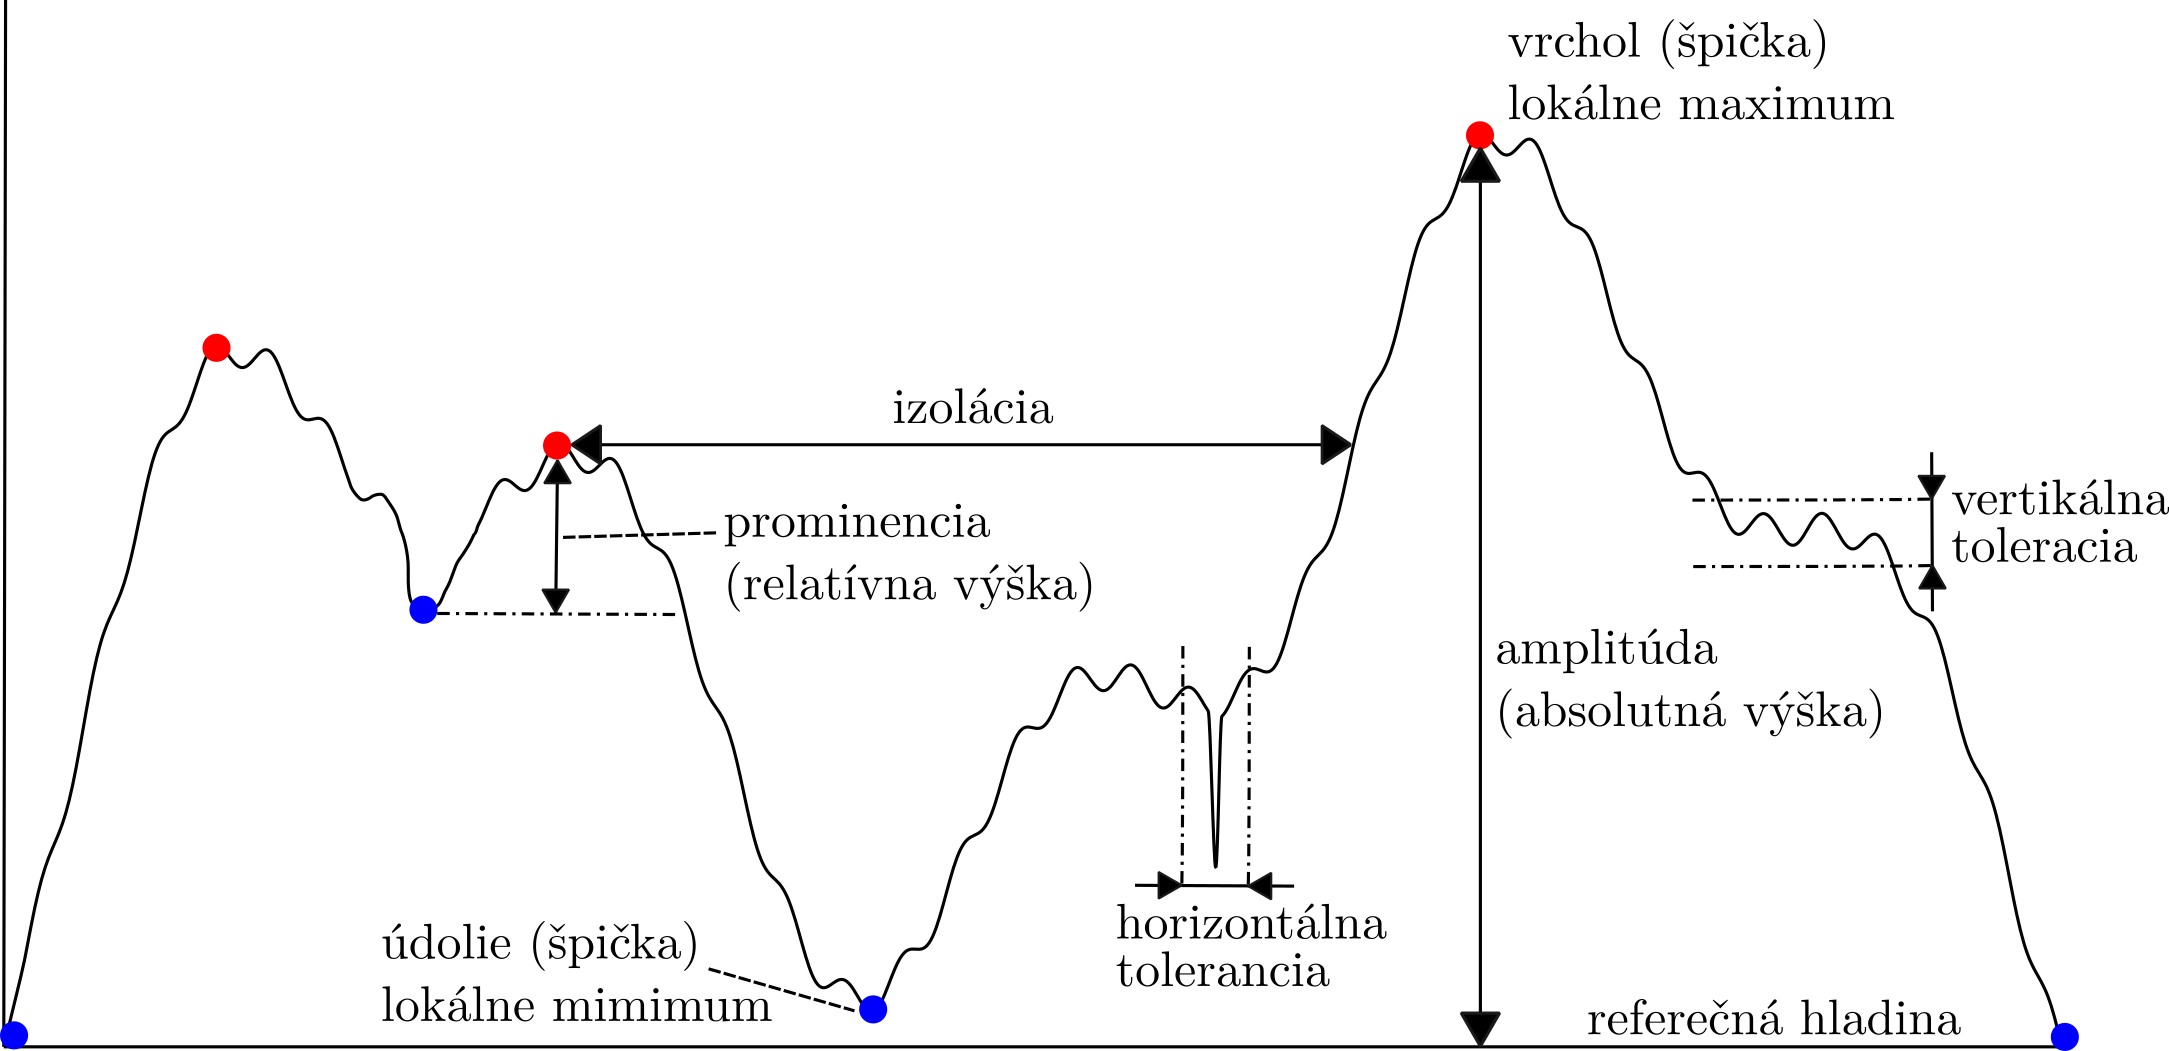
\includegraphics[width=0.9\textwidth]{figures/topography.png}
    \caption{Topografia priebehu signálu}
    \label{fig:topography}
\end{figure}

Domnelý vrchol je označený za lokálne maximum, keď spĺňa parametre pre topografické vlastnosti minimálnej akceptovateľnej
prominencie a izolácie (obr. \ref{fig:topography}. Prominencia znamená relatívnu výšku oproti predošlej navštívenej doline. Izolácia vyčísľuje vzdialenosť k najbližšiemu skoršiemu vrcholu. Podobný algoritmus už existuje v literatúre \cite{peek-mountaineer-method}, avšak nižšie prezentovaný pseudokód je oproti nemu zjednodušený a doplnený o požadované tolerancie.
\begin{algorithm}[h]
\caption{Algoritmus horského turistu}
\begin{algorithmic}[1]
\Function{Find\_Peaks\_Hill\_Walker}{$y$, $tolerance$, $hole$, $prominence$, $isolation$}
	\State $peaks \gets []$
	\State $i\_change \gets 0$
	\State $y\_valley \gets 0$
	\State $possible\_change \gets false$
	\State $uphill \gets (y[1] - y[0]) \geq 0$

	\For{$i \gets 1$ \textbf{to} $length(y)$}
		\State $y\_step \gets y[i] - y[i-1]$
        \State $slope \gets y\_step \geq 0$

        \If {$possible\_change = false$ \textbf{and} $uphill \neq slope$}
        	\State $possible\_change \gets true$   \Comment{Označenie potenciálneho extrému}
        	\State $i\_change \gets i - 1$
        \ElsIf {$possible\_change = true$ \textbf{and} $uphill = slope$}
        	\State $possible\_change \gets false$  \Comment{Potenciálny extrém bol zachvením}
        \EndIf

        \If {($possible\_change = true$
        	\State \hskip1.5em \textbf{and} $uphill \neq slope$
        	\State \hskip1.5em \textbf{and} $|i - i\_change| > hole$
        	\State \hskip1.5em \textbf{and} $|y[i] - y[i\_change]| > tolerance$)}

        	\State $posible\_change \gets False$        \Comment{Významný lokálny extrém potvrdený}
        	\State $prev\_uphill \gets uphill$
        	\State $uphill \gets slope$

        	\If {$prev\_uphill = false$ \textbf{and} $uphill = true$}
				\State $y\_valley \gets y[i\_change]$   \Comment{Nájdené údolie}

            \ElsIf {($prev\_uphill = true$
            		\State \hskip1.5em \textbf{and} $uphill = false$
            		\State \hskip1.5em \textbf{and}  $|y[i - hole] - y\_valley| > prominence$)
            		\State \hskip1.5em \textbf{and}  $|y[i - hole] - y[last(peaks)]| > isolation$)}
				\State $y\_peak \gets y[i\_{change}]$    \Comment{Skutočný vrchol identifikovaný}
				\State $peaks \gets peaks + [i_{change}]$
            \EndIf
        \EndIf
	\EndFor
	\State \Return $peaks$
\EndFunction
\end{algorithmic}
\label{algo:mountain-hiker}
\end{algorithm}
\afterpage{\clearpage}

\subsection{Metriky pre binárny klasifikátor}
Uviedli sme tri rozdielne rovnocenné prístupy odhalenia špičiek. Rozobrali sme algoritmus porovnávajúci susedov na obe strany,
algoritmus využívajúci sklon sečníc vychádzajúc s vlastností prvej derivácie a napokon
stavový automat odvolávajúci sa na sekvenčne preskúmavanú topografiu krivky grafu. Spoločným rysom zmienených techník
je vykonávanie binárne zaradenie pre každú vzorku, či sa sa nachádza alebo nenachádza na aktuálnej pozícii vrchol.

Rozhodnutie môže viesť k správnemu ($P$) alebo nesprávnemu ($N$) riešeniu vzhľadom na objektívnu pravdu
sprostredkovanú anotovanými dátami. Keď sa kategorizácia zhoduje s realitou dostávame skupiny
skutočne pozitívnych $TP$ a skutočne negatívnych $TN$. V prípade, že sa klasifikátor pomýli vyjde buď chyba
prvého rádu $FP$, kedy registrujeme neexistujúcu špičku, alebo chyba druhého rádu $FN$, kedy ju prehliadneme.
Umiestnením počtov charakteru rozhodnutí do tabuľky vzniká matica zámen \cite{binary-classifier}.

Úspešnosť klasifikačných algoritmov pre ich vzájomné porovnanie kvantifikujú viaceré metriky. Na odladenie parametrov
vplývajúcich na náchylnosť preferovať kladné alebo záporné výsledky sa vzťahuje \emph{prevalencia} výskytu očakávaného
javu: $P / (P+N)$ v samotných dátach. Snahou rozhodovania je maximalizovať senzitivitu a špecifickosť výsledkov algoritmu.
\emph{Senzitivita} (\ref{equ:sensitivity}) udáva koľko bodov, ktoré sú prehlásené za špičky naozaj je špičkami.
\emph{Špecifickosť} (\ref{equ:specifity}) sa zameriava na potvrdenie, aké množstvo pozorovaní nepovažovaných za špičky,
nie sú nimi aj skutočne.
\myequations{Metriky klasifikátora: senzitivita a špecifickosť}
\begin{ceqn}\begin{align}
TPR = \frac{TP}{P} = \frac{TP}{TP + FN} \label{equ:sensitivity} \\
TNR = \frac{TN}{N} = \frac{TN}{TN + FP} \label{equ:specifity}
\end{align}\end{ceqn}

Presnosť určenia lokálneho extrému sa skladá z správnosti (\ref{equ:ppv}) a precíznosti (\ref{equ:accuracy}),
ktoré je rovnako žiaduce dosahovať čo najbližšie sto percentám, pri nízkej chybovosti (\ref{equ:error-rate}), čiže
nízkeho počtu falošných poplachov.
\myequations{Metriky klasifikátora: správnosť, precíznosť, chybovosť}
\begin{ceqn}\begin{align}
PPV = \frac{TP}{TP + FP} \label{equ:ppv} \\
ACC = \frac{TP + TN}{P + N}\label{equ:accuracy} \\
FPR = \frac{FP}{FP + TN} \label{equ:error-rate}
\end{align}\end{ceqn}

Štandardným nástrojom na vyjadrenie kvality binárneho klasifikátora je \emph{ROC krivka} zakresľujúca
senzitivitu $TPR$ vo zvislom smere voči vodorovnej chybovosti $FPR$. ROC vytvoríme postupným posúvaním prahu
pre klasifikáciu prostredníctvom parametrov algoritmu. Použiteľný algoritmus sa vyznačuje vypuklou krivkou
smerom k ľavému hornému rohu nad diagonálou, ktorá by sprevádzala počínanie náhodného rozhodovania. Dokonalá
metóda pri dosahovala stopercentnú senzitivitu za nulovej chyby. Vyjadrením plochy pod
ROC krivkou je miera AUC, ktorá umožňuje približné číselné porovnanie rôznych získaných kriviek \cite{roc-analysis}.

\section{Frekvenčná a časovo-frekvenčná analýza signálu}
Cyklicky sa opakujúce deje v signále sú extrahované zo sekvencie vzoriek v časovej doméne transformovaným do domény frekvenčnej.
Premenou dochádza k odhadu sumárnej intenzity jednotlivých rozsahov zložiek spektra, pričom rozlíšenie je
podmienené vzorkovacou frekvenciou $f_s$ a celkovým počtom meraní $N$ (\ref{equ:freq-resolution}) \cite{understanding-dsp}.
\myequations{Rozlíšenie vo frekvenčnej domény podľa vzorkovania}
\begin{ceqn}\begin{align}
\Delta f = \frac{f_s}{N} \label{equ:freq-resolution}
\end{align}\end{ceqn}

Kompromis potrebný učiniť pri spektrálnej analýze tkvie vo vyvážení dĺžky úseku pre časovú lokalizáciu frekvenčného obrazu,
a jeho výslednej detailnosti na strane druhej. Prechod medzi časovou a frekvenčnou doménou postihuje princíp neurčitosti
znamenajúci, že pri raste rozlíšenia v čase strácame rozlíšenie vo frekvenciách a naopak \cite{signal-processing}.
O požadovanom množstve pozorovaní pre konkrétnu rozlíšiteľnosť spektra taktiež hovorí vzťah (\ref{equ:freq-resolution}).
Rozpätie frekvencií spadajúcich do diskrétneho frekvenčného vedierka $k$ sú počínajúc $k\Delta f$ po $(k+1)\Delta f$.

\subsection{Diskrétna fourierová a kosínusová transformácia}
Diskrétna Fourierová transformácia (DFT) slúži na učenie harmonického zloženia signálu (\ref{eq:dft}) rozkladom na súčet
sínusov a kosínusov rôznych frekvencií. Zobrazuje vektor komplexných čísel $y$ dĺžky $N$ do vektora $N$ frekvenčných
komponentov. Na vypočítanie $k$-teho frekvenčného vedierka sú
prvky sekvencie pozorovaní prenásobené zodpovedajúcim exponenciálnym členom tzv. \emph{twiddle factor} (\ref{eq:twiddle}). Inverzná
transformácia sa líši iba opačným znamienkom exponenta a získané hodnoty sa zvyknú normovať podelením $N$.
\myequations{Diskrétna Fourierová transformácia}
\begin{ceqn}\begin{align}
Y[k] &= \sum_{n=0}^{N - 1}{x[n] \cdot W_N^{nk}};\quad k = 0, \dots, N - 1 \label{eq:dft}\\
W_{N}^{nk} &= \exp{\left(-i2\pi nk \, /\, N\right)} \label{eq:twiddle}
\end{align}\end{ceqn}

Alternatívne exponenciálny faktor vyjadruje v goniometrickom tvare ako kosínusovú reálnu časť a sínusovú imaginárnu časť:
\myequations{Exponenciálny faktor pre DFT v goniometrickom tvare}
\begin{ceqn}\begin{align}
W_{N}^{nk} = \cos(2\pi nk/ N) - i \cdot \sin(2\pi nk/ N)
\end{align}\end{ceqn}

Spektrálne komponenty opísané vektorom komplexných Fourierových koeficientov majú magnitúdy dané veľkosťami komplexných čísel
(\ref{equ:magnitude-spectrum}). Pre vstupy $x \in \mathcal{R}$ je výstup z DFT zrkadlovo symetrický, čiže druhá polovica
výstupu je komplexne združená k prvej $x[m] = x^{*}[N - m]$. Symetrickosť zapríčiňuje nadbytočnosť výsledkov
nad pozíciou  $N/2$. Rovnako naznačuje reformulácia vety o vzorkovaní, že za vzorkovacej frekvencie $f_s$ sú zapríčinením aliasingu v signále prítomné frekvencie do maximálne polovice $f_s$. Energia vo frekvenčnom vedierku je druhou mocninou magnitúdy, ale častejšie sa
objavuje reprezentácia relatívneho energetického spektra v decibeloch (\ref{equ:decibel-spectrum}) \cite{understanding-dsp}.
\myequations{Magnitúdové spektrum absolútne a relatívne v decibeloch}
\begin{ceqn}\begin{align}
|Y[k]| = \sqrt{\Re\{Y[k]\}^2 + \Im\{Y[k]\}^2} \label{equ:magnitude-spectrum} \\
Y_{dB}[k] = 20 \cdot \log_{10}{ \left( \frac{|Y[m]|}{\max\{|Y[m]|\}} \right)} \label{equ:decibel-spectrum}
\end{align}\end{ceqn}

Sekvencia pozorovaní vyjadrená cez súčet kosínusoid namiesto exponenciálneho faktora tvorí rodinu diskrétnych
kosínusových transformácií (DCT). Vyznačujú sa dobrou dekoreláciu vstupu a energetickou kompresiou, čiže pomerne veľká
časť celkovej spektrálne energie je sústredená v málo koeficientoch \cite{dct-applications}. Navyše oproti DFT umožňuje redukciu
výpočtovej náročnosti odstránením súčinov v komplexných číslach.

Podľa charakteru obmien kosínusovej bázy rozlišujeme
štyri typy DCT,  z nich najvýznačnejšie sú transformácie DCT-II, ktorej inverziou je DCT-III, a DCT-IV, ktorá je inverzná
sama sebe \cite{dct}. Z DCT-IV vychádza MDCT, ktorá navyše spracováva prekrývajúce sa bloky, tak že druhá polovica vzoriek
pochádza z prvej polovice ďalšieho bloku. Dokopy vytvorí z $2N$ vzoriek $N$ koeficientov. MDCT sa hojne využíva pri stratovej
kompresii zvuku, pretože sa prelínaním blokom vyvaruje artefaktom na hraniciach blokov
\cite{mdct}.
\myequations{Kosínusové transformácie: DCT-II, DCT-III, DCT-IV, MDCT}
\begin{ceqn}\begin{align}
\tag{DCT-II} W_{N}^{nk} &= \cos{\left[\left(n + \frac{1}{2}\right) k\frac{\pi}{N}\right]} \\
\tag{DCT-III} W_{N}^{nk} &= \cos{\left[n \left(k + \frac{1}{2} \right) \frac{\pi}{N}\right]}  \\
\tag{DCT-IV} W_{N}^{nk} &= \cos{\left[\left(n + \frac{1}{2} \right) \left(k + \frac{1}{2} \right) \frac{\pi}{N} \right]} \\
\tag{MDCT} W_{N}^{nk} &= \cos{\left[\left(n + \frac{1}{2} + \frac{N}{2} \right) \left(k + \frac{1}{2} \right) \frac{\pi}{N} \right]};\quad n = 0, \dots, 2N - 1
\end{align}\end{ceqn}

\subsection{Algoritmus FFT}
Priamočiarou implementáciou vzťahom na výpočet Fourierovej a kosínusovej transformácie dosiahneme časovú zložitosť
rádu $\mathcal{O}(N^2)$. Aplikáciam v reálnom čase na prúdoch dát takáto výpočtová náročnosť zďaleka nepostačuje.
Algoritmus rýchlej fourierovej transformácie (FFT) uplatňujúci prístup rozdeľuj a panuj zvládne zrealizovať DFT
v čase $\mathcal{O}(N \log N)$.

Celkovo pozostáva z $N$ sčítaní a $N/2$ násobení v komplexných číslach. Najbežnejšia
varianta algoritmu FFT radix-2 vyžaduje, aby veľkosť vstupu bol mocninou dvojky: $N = 2^k$ .
Značná výpočtová úspora sa nadobúda uvažovaním s periodicitou goniometrických funkcií pri twiddle faktoroch $W_N$ a z
toho vyplývajúcich symetrií Fourierovej matice, keďže len $N$ z $N^2$ prvkov matice je odlišných \cite{fft-blackbox}.

Podľa spôsobu dekompozície vstupného vektora sú známe dve verzie Radix-2 FFT nazvané decimácia v čase (DIT)
a decimácia vo frekvencii (DIF). Decimácia v čase (obr. \ref{fig:dit-fft}) rekurzívne delí hodnoty na párne a
nepárne pozície v čase, zatiaľ  čo decimácia vo frekvencii (obr. \ref{fig:dif-fft}) rozdeľuje na tieto na párne a
nepárne frekvenčné vedierka \cite{dit-dif-fft}. Výpočet prebieha v $\log_2(n)$ deliacich fázach. Poradie prvkov
vo výstupnom vektore je vždy bitovo invertované, čiže poradové číslo zapísané ako bitový reťazec má obrátené
poradie. Na dosiahnutie výstupu poradí rastúcich pozícií musí byť pred spustením FFT vstup preusporiadaný
\cite{computer-vision-fft}.

\begin{figure}[h]
\centering
\begin{subfigure}[b]{0.48\textwidth}
    \centering
    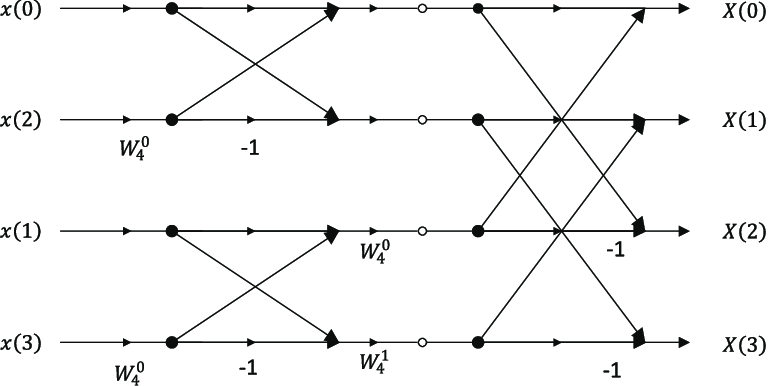
\includegraphics[width=\textwidth]{figures/Length-4-DIT-radix-2-FFT.png}
    \caption{Decimácia v čase}
    \label{fig:dit-fft}
\end{subfigure}
\hfill
\begin{subfigure}[b]{0.48\textwidth}
    \centering
    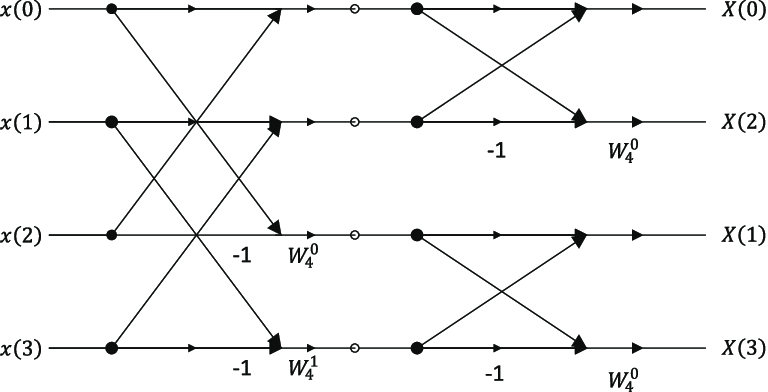
\includegraphics[width=\textwidth]{figures/Length-4-DIF-radix-2-FFT.png}
    \caption{Decimácia vo frekvencii}
    \label{fig:dif-fft}
\end{subfigure}
\caption{Radix-2 FFT na štyroch bodoch \cite{dit-dif-fft}}
\end{figure}

Základným prvkom schémy výpočtu je motýlikový diagram (,,butterfly''), ktorý je odlišný pre DIT (obr. \ref{fig:dit-butterfly})
a pre DIF verziu (obr. \ref{fig:dif-butterfly}). Motýlik obsahuje vynásobenie
jedného z príchodzích operandov s vopred vypočítaným exponenciálnym členom $W_N^j$ pre $j = 0, ..., N/2 - 1$
\cite{fft-blackbox}, a následné prirátanie a tiež odpočítanie od druhého operandu.

\begin{figure}[h]
\centering
\begin{subfigure}[b]{0.48\textwidth}
    \centering
    
\includegraphics[width=\textwidth]{figures/dit-butterfly.png}
    \caption{Decimácia v čase}
    \label{fig:dit-butterfly}
\end{subfigure}
\hfill
\begin{subfigure}[b]{0.48\textwidth}
    \centering
    
\includegraphics[width=\textwidth]{figures/dif-butterfly.png}
    \caption{Decimácia vo frekvencii}
    \label{fig:dif-butterfly}
\end{subfigure}
\caption{Motýlikové diagramy algoritmu FFT}
\end{figure}

Efektívnejšie na celkový počet aritmetický počet operácií oproti FFT s radixom 2 je \emph{split-radix}, ktorý
kombinuje výhody vyplývajúce z radix-4 pre nepárne členy DFT a radix-2 pre párne členy. Veľkosť vstupného
vektora musí byť násobkom štyroch. Dosahuje okolo 30\% zníženie počtu násobení a 10\% pokles počtu sčítaní
oproti radix-2 \cite{split-radix}.

Algoritmus FFT je aplikovateľný taktiež na výpočet DCT vhodným zoradením vstupného vektora. DCT-II $N$-bodovej
reálnej postupnosti $\mathbf{x}$ sa odvodzuje uskutočnením jej $2N$-bodového párneho rozšírenia a vynásobenie výsledku
twiddle faktorom $2W_{2N}^{k}$ a ponechaní reálnej časti. Na ilustráciu uvádzame prípad
DCT 4-bodovej sekvencie $(x_1, x_2, x_3, x_4)$, ktorej párnym rozšírením $\mathbf{y}$ je $(x_1, x_2, x_3, x_4, x_4, x_3, x_2, x_1)$.
Rovnako by postačovalo vyplniť pôvodnú postupnosť nulami do dĺžky $2N$, čiže dostávame $(x_1, x_2, x_3, x_4, 0, 0, 0, 0)$.
Postačuje však realizovať $N$-bodovú FFT sekvencie párnych alebo nepárnych prvkov z $\mathbf{y}$, ktoré sú vzájomným reverzom.
Na základe predošlého predošlého príkladu dostaneme postupnosť $(x_1, x_3, x_4, x_2)$ \cite{fast-dct}.

Široké použitie FFT pri spracovaní signálov sa prejavuje dostupnosťou implementácií rôznych obmien algoritmu
v širokej škále programovacích jazykov a optimalizované pre konkrétne hardvérové platformy. V jazyku C stoja
za zmienku knižnice: FFTW, FFTPACK, GNU Scientific Library, CMSIS DSP a Espressif DSP. Na účely analýzy údajov je FFT
prítomné pre jazyk Python v balíkoch \emph{numpy} a \emph{scipy}, tiež napr. v jazyku R je súčasťou \emph{stats} modulu.

\subsection{Oknové funkcie}
U stochastického signálu má zmysel delenie na rovnako dlhé úseky, pretože sa s časom mení jeho spektrálny obsah, ktorý
je žiaduce zachytiť čo najpresnejšie. Krátkodobá Fourierová transformácia zahŕňa preto ováhovanie meraní
v časovej doméne koeficientmi posuvnej oknovej funkcie. Mimo intervalu pôsobnosti okna sú vzorky vynulované.

DFT predpokladá periodicitu časového radu do nekonečna, preto ak frekvencia sínusového vstupu nie je presným násobkom
frekvenčného rozlíšenia, čiže priebeh exaktne nepripadá frekvenčnému vedierku, dochádza k úniku spektra (spectral leakage).
Prejavom je hraničný efekt pre odlišnosť poslednej a prvej vzorky, ktorá je považovaná za nespojitosť a prejavuje
sa zvlnením v okolí diskontinuity podľa Gibsovho javu \cite{understanding-dsp}.

Existuje množstvo oknových funkcií líšiacich sa mierou kompromisu medzi šírkou výsledných špičiek vo frekvenčnej doméne,
presnosti v amplitúde a spôsobu poklesu úniku spektra do ostatných vedierok. Medzi najpoužívanejšie sa zaraďujú: obdĺžníkové
(\ref{equ:window-rectangular}), Bartlettovo (\ref{equ:window-bartlett}), Hannovo (\ref{equ:window-hann}), Hammingovo
(\ref{equ:window-hamming}) a Blackmannovo okno \ref{equ:window-blackmann}. Uvedené okná sú stredovo súmerné (obr. \ref{fig:window-time})
Plochejšie okná, napríklad obdĺžníkové, sa vyznačujú ponechaním ostrejších špičiek s neskreslenou amplitúdou za
cenu väčšieho spektrálneho úniku, čím sa znižuje odstup od šumu. Predchádzanie hraničným javom sa dosahuje plynulým
znižovaním hodnôt k okrajom okna až na nulu, čím špičky strácajú na amplitúde (scalloping loss) \cite{spectral-density-estimation}.
\myequations{Oknové funkcie: obdĺžník, Bartlett, Hann, Hamming, Blackman}
\begin{ceqn}\begin{align}
w(n) &= 1,\, n = 0, 1, ..., N - 1 \label{equ:window-rectangular} \\
w(n) &= \frac{2}{N - 1}\left(\frac{N - 1}{2} - \left|n - \frac{N - 1}{2} \right|\right) \label{equ:window-bartlett}  \\
w(n) &= \cos^2((2\pi n / N - \pi) / N)  \label{equ:window-hann} \\
w(n) &= 0.54 - 0.46\cos(2\pi n / N) \label{equ:window-hamming} \\
w(n) &= 0.42 - 0.5\cos(2\pi n / N) + 0.08\cos(4\pi n / N)\label{equ:window-blackmann}
\end{align}\end{ceqn}

Fourierou transformáciou okna dostávame frekvenčnú odozvu, ktorá má tvar funkcie $\mathrm{sinc}(x) = \sin(x) / x$
(obr. \ref{fig:window-freq}) Priebeh odozvy sa vyznačuje hlavným a vedľajšími vrcholmi (mainlobe a sidelobes).
Hlavný vrchol sa snažia
rôzne oknové funkcie udržať čo najužší, lebo zodpovedá za šírku spektrálneho úniku do okolitých vedierok.
Vedľajšie vrcholy sú nežiaduce a podmieňujú najmä úroveň odstupu od šumu.

\begin{figure}[h]
\centering
\begin{subfigure}[b]{0.48\textwidth}
    \centering
    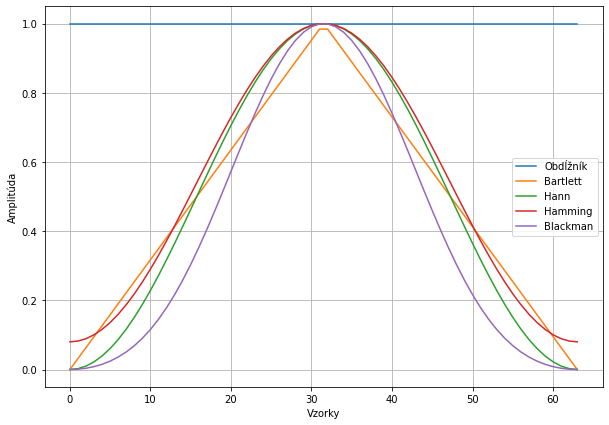
\includegraphics[width=\textwidth]{figures/window-time.png}
    \caption{Časový priebeh}
    \label{fig:window-time}
\end{subfigure}
\hfill
\begin{subfigure}[b]{0.48\textwidth}
    \centering
    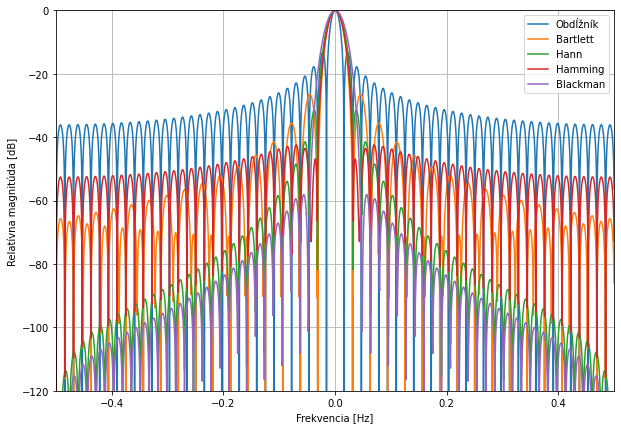
\includegraphics[width=\textwidth]{figures/window-freq.png}
    \caption{Frekvenčná odozva}
    \label{fig:window-freq}
\end{subfigure}
\caption{Tvar oknových funkcií s dĺžkou $N = 31$}
\end{figure}

Vzhľadom na skutočnosť, že oknové funkcie sa typicky blížia nule smerom k okrajom, bola by veľká časť pozorovaní
časového radu ignorovaná. Prekrývaním okien vo vhodnom pomere je umožnený rovnomerný vplyv
hodnôt, ktoré pripadnú na okraj niektorého okna. Pomer sa stanovuje štandardne
na 50\%, aj s ohľadom na rastúcu výpočtovú záťaž s väčším prekrývaním. Výnimkou je obdĺžníkové okno kde to nemá
zmysel. Platí, že pri iných užších oknách je potrebné rátať s väčším presahovaním ako pri širších. Vyhodnotenie veľkosti
prekrývania sa zakladá na korelácii spektrogramov a plochosti amplitúdy, čiže pomeru minimálnej váhy na pozorovanie
vo všetkých oknách ku maximálnej dosiahnutej amplitúde ideálne rovnajúce sa jednotke \cite{spectral-density-estimation}.

Jediný odhad frekvenčných zložiek postupnosti vzoriek vedie k vysokej neurčitosti odhadov pre frekvenčné vedierka,
keďže smerodajná odchýlka odhadu je totožná s odhadom samotným \cite{spectral-density-estimation}. Welchova metóda
spriemerovania upravených periodogramov spresní úrovne frekvencií cez priemer viacerých prekrývajúcich
sa energetických spektier \cite{welch-method}.

\subsection{Filtre s konečnou impulznou odozvou}
Predspracovanie signálu do podoby vhodnejšej na analýzu, extrakciu čŕt a detekciu udalostí sa vykonáva filtrovaním.
Častými činnosťami býva odstránenie posunu alebo jednosmernej zložky, eliminovanie šumu rozptýleného medzi
vysokofrekvenčné komponenty, a oddelenie známeho frekvenčného pásma od zvyšku spektra. Dolná priepusť prepustí
nízke frekvencie až po medznú frekvencie, od ktorej nahor frekvencie utlmuje. Horná priepusť sa správa opačne
a potláča nižšie frekvencie. Pásmová priepusť ponechá frekvencie v obmedzenom rozsahu z oboch strán.

Ideálne filtre majú okamžitý útlm dovoľujúci prechod striktne vymedzeným zložkám signálu. Vo frekvenčnej doméne
oblasti nadobúdajú preto tvar obdĺžníkového okna. Transformáciou do časovej domény sa obdĺžník zmení
na konvolučnú masku, resp. impulznú odozvu $h[k]$, s priebehom $\mathrm{sinc}$ funkcie, ktorá nie je vyjadriteľná nekonečne
presne, čím vznikajú prechodové javy vo frekvenčnej odozve filtra a menšia strmosť útlmu s kratším filtrom.

Konečná impulzná odozva v názve FIR filtra znamená, že pri vyjadrení filtra sa obmedzíme na konečný počet
koeficientov orezaním impulznej odozvy rovného rádu filtra $k$. Výpočet upravenej hodnoty sa v časovej doméne počíta
ako diskrétna konvolúcia s časovou zložitosťou $\mathcal{O}(nk)$, pre časový rad dĺžky $n$. Diagram výpočtu je zachytený
na obr. \ref{fig:fir-filter}.
\myequations{Výpočet FIR filtra cez konvolúciu}
\begin{ceqn}\begin{align}
y[n] = x[n] * h[n] = \sum_{i=0}^{K}{h[i] \cdot x[n - i]}
\end{align}\end{ceqn}

Masky dolnej (\ref{equ:low-pass}), hornej (\ref{equ:high-pass}) a pásmovej priepuste (\ref{equ:band-pass}) popisujú
uvedené vzťahy pre medznú normalizovanú frekvenciu $f_c = f / f_s$ a $n = -k/2, \dots, 0, \dots, k/2$. Zvlnenie v prechodovom pásme
medzi rozsahmi so ziskom a útlmom je vylepšené návrhom filtra za použitia oknovej funkcie (napr. Blackman) na žiadanú
frekvenčnú odozvu.
\myequations{Koeficienty FIR filtra pre dolnú, hornú a pásmovú priepusť}
\begin{ceqn}\begin{align}
h_{LPF}[n] &= \mathrm{sinc}(2 f_c n)  \label{equ:low-pass} \\
h_{HPF}[n] &= (-1)^n \cdot h_{LPF}[n] \label{equ:high-pass} \\
h_{BPF}[n] &= \mathrm{sinc}(2 f_{c2} n) -  \mathrm{sinc}(2 f_{c1} n)  \label{equ:band-pass}
\end{align}\end{ceqn}

Podľa konvolučnej vety platí, že konvolúcia v čase je násobením vo frekvenciách, umožňujúc urýchlenie filtrovania
pre veľké masky. Kým vtedy sa blíži zložitosť konvolúcie ku kvadratickej, na násobenie vo frekvenčnej doméne so
stačí vykonať FFT a IFFT dohromady v rádovo $\mathcal{O}(n \log n)$.

\begin{figure}[h]
	\centering
	
\includegraphics[width=0.8\textwidth]{figures/fir-filter.png}
	\caption{Bloková schéma FIR filtra rádu $k$}
	\label{fig:fir-filter}
\end{figure}

\section{Senzorová sieť}
Zber údajov meraní z prostredia zabezpečujú samočinné senzorové jednotky schopné dlhodobej prevádzky
často za vystavenia nepriaznivým okolitým podmienkam. Hlavnou limitáciou prevádzky senzoriky je spotreba energie,
pretože doba funkčnosti zariadenia ohraničuje kapacita batérií, ktoré sú obtiažne vymeniteľné pri nasadení
v nedostupných lokalitách alebo pozíciach. Senzor musí byť ideálne schopný autonómnej konfigurácie
reakciou na zmenu nastatých okolností a s tým súvisí zotavenie z neočakávaných a chybových stavov \cite{wsn-overview}.

Výpočtový výkon býva za cenu zníženia elektrického odberu redukovaný
znížením taktovacej frekvencie a snahou efektívny manažment periférií distribúciou hodín a dostupnými
úspornými režimami. Menej dostupných cyklov procesora povoľuje realizáciu jednoduchších výpočtov, ktoré zväzuje
u niektorých aplikácií nutnosť odozvy v reálnom čase. Aby sa zachovala nízka cena zariadení šetrí sa
na lokálne dostupnom úložisku, ktoré sa počíta v kilobajtoch nanajvýš megabajtoch.

Senzorové jednotky si buď získané dáta ukladajú na externú flash pamäť, alebo sa od nich vyžaduje komunikácia
cez bezdrôtové spojenie. Prepojením na internet sa zaraďujú k zariadeniam Internetu vecí (IoT).
Na rýchlosť sieťového prenosu má dopad okrem šírky pásma a réžie protokolov
vzdialenosť od sieťovej brány v prípade hviezdicovej topológie alebo najbližšieho susedného uzla v mesh
alebo point-to-point rozložení. Vynaloženým výkonom na príjem a vysielanie je postihnutý dosah, ktorý
ovplyvňujú aj prekážky na trase a iné interferencie. Štandardne používané bezdrôtové technológie
v pásmach ISM sú uvedené v tabuľke \ref{tab:net-protocols}.

\begin{table}[h]
\centering
\def\arraystretch{1.2}
\begin{tabular}{|l|r|rr|r|}
\hline
\textbf{\begin{tabular}[c]{@{}l@{}}Bezdrôtový\\ protokol\end{tabular}} & \multicolumn{1}{l|}{\textbf{\begin{tabular}[c]{@{}l@{}}Frekvenčné\\ pásmo v EÚ\end{tabular}}} & \multicolumn{1}{l|}{\textbf{\begin{tabular}[c]{@{}l@{}}Prenos\\ max.\\ (Mbit/s)\end{tabular}}} & \multicolumn{1}{l|}{\textbf{\begin{tabular}[c]{@{}l@{}}Prenos\\ typ.\\ (Mbit/s)\end{tabular}}} & \multicolumn{1}{l|}{\textbf{\begin{tabular}[c]{@{}l@{}}Dosah\\ cca\\ (m)\end{tabular}}} \\ \hline
Bluetooth LE 4                                                                   & 2,4 GHz                                                                                       & \multicolumn{1}{r|}{1}                                                                         & 0,3                                                                                            & 10 - 30                                                                                 \\ \hline
Bluetooth LE 5                                                                   & 2,4 GHz                                                                                       & \multicolumn{1}{r|}{2}                                                                         & 1,3                                                                                            & 30 - 50                                                                                 \\ \hline
Wifi: 803.11 b                                                                   & 2,4 GHz                                                                                       & \multicolumn{1}{r|}{11}                                                                        & 5                                                                                              & 35 - 140                                                                                \\ \hline
Wifi: 803.11 n                                                                   & 2,4 GHz                                                                                       & \multicolumn{1}{r|}{54}                                                                        & 25                                                                                             & 35 - 140                                                                                \\ \hline
Wifi: 803.11 g                                                                  & 2,4 / 5 GHz                                                                                   & \multicolumn{1}{r|}{300 / 600}                                                                 & 150                                                                                            & 70 - 250                                                                                \\ \hline
ZigBee: 802.15.4                                                                 & \begin{tabular}[c]{@{}r@{}}868 MHz\\ 2,4 GHz\end{tabular}                                     & \multicolumn{2}{r|}{\begin{tabular}[c]{@{}r@{}}20 kbit/s\\ 250 kbit/s\end{tabular}}                                                                                                             & 10 - 100                                                                                \\ \hline
Z-Wave                                                                           & 868 MHz                                                                                       & \multicolumn{2}{r|}{40 - 100 kbit/s}                                                                                                                                                            & 30 - 100                                                                                \\ \hline
LoRaWAN                                                                          & 863 MHz                                                                                       & \multicolumn{2}{r|}{0,3 - 50 kbit/s}                                                                                                                                                            & 5 - 20 km                                                                               \\ \hline
Narrowband IoT                                                                   & \multicolumn{1}{l|}{Operátor}                                                                 & \multicolumn{2}{r|}{250 kbit/s}                                                                                                                                                                 & \multicolumn{1}{l|}{1 - 10 km}                                                          \\ \hline
\end{tabular}
\caption{Prehľad najpoužívanejších typov sietí pri IoT komunikácii}
\label{tab:net-protocols}
\end{table}

Na harmonizáciu využívania rádiového frekvenčného spektra pre zariadenia s krátkym dosahom sa v
Slovenskej republike vzťahuje vykonávacie rozhodnutie Komisie Európskej únie 2019/1345. Definujú sa
tam voľné frekvenčné pásma s povoľovaním príslušného maximálneho legálneho vysielacieho výkonu
zariadení \cite{eu-frequencies}.

V Sub-1 GHz oblasti je k dispozícii rozsah 863 - 870 MHz využívaný LPWAN (Low-Power Wide Area Network) obmedzený
časom vysielania na 0.1\%, 1\%, alebo 10\% z hodiny a výkonom do 25 mW. Wifi (IEEE 803.11) a Bluetooth zaberajú
rozsah 2400 - 2 483,5 MHz s povoleným výkonom do 100 mW na 100 KHz. Protokoly
ako Bluetooth sa navyše označujú triedami podľa ponúkaného dosahu. Trieda 1 deklaruje dosah do 100 metrov za výkonu
do 100 mW, trieda 2 je približne do 10 metrov a do 2,5 mW a trieda 3 je na 1 meter a 1 mW \cite{bluetooth}.
IoT tiež využíva na komunikáciu mobilné siete poskytované operátormi (napr. NB-IoT, GPRS, 3G, 4G/LTE a 5G),
tam sú frekvencie licencované.

Operácia uzlov sa rozdeľuje podľa podnecujúceho činiteľa ako založené na udalostiach (event-driven),
dopytoch (query-driven) alebo čase (time-driven) \cite{big-data-collection-wsn}. Event-driven
nepretržite vyhodnocuje vstupy ale upozorní až po zachytení náhlej zmeny alebo prekročení prahovej úrovne.
Query-driven systém reaguje na aktuálne požiadavky od používateľa a odpovie so sadou dát zodpovedajúcej požiadavke.
Time-driven systém pravidelne odosiela zozbierané údaje do siete podľa nastavení od riadiaceho uzla.

IoT zariadenia na okrajoch siete vytvárajú veľký objem dát, ktorý sa tradične posiela na zhromaždenie, spracovanie
a analýzu na centrálny server alebo do cloudu. Posunom paradigmy s cieľom vyhodnotenia dát, čo najbližšie
ku zdroju dát za zníženia latencie pri spracovaní, sieťovej premávky a záťaže na cloudové riešenie, a zvýšením
bezpečnosti sa rozširuje edge computing (,,počítanie na okraji'').
\begin{figure}[h]
	\centering
	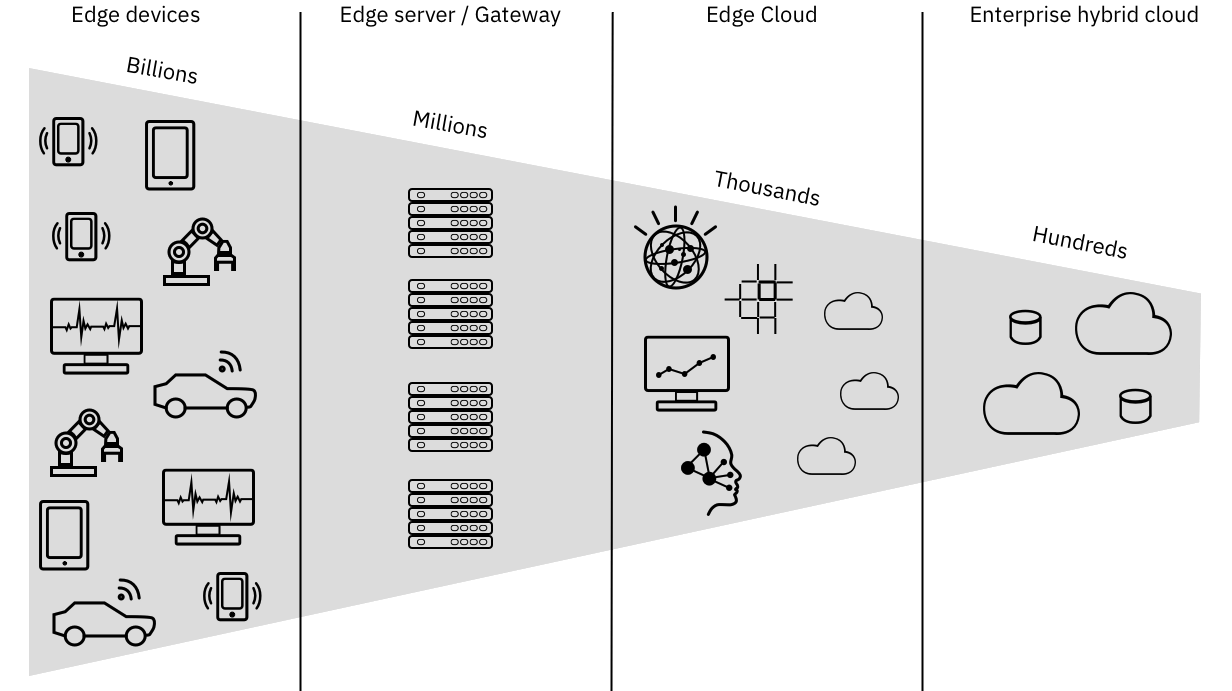
\includegraphics[width=0.9\textwidth]{figures/edge-computing.png}
	\caption{Prvky architektúry Edge computing \cite{ibm-edge-architecture}}
	\label{fig:fir-filter}
\end{figure}

Edge computing je viacvrstvová distribuovaná architektúra vyvažujúca zodpovednosti a záťaž medzi
tri vzájomne sa dopĺňajúce úrovne: Device edge, Local edge a Cloud \cite{edge-computing-survey}. Na okraji sieti
vrámci device edge pôsobia  samotné IoT zariadenia získavajúce dáta z fyzických veličín prostredia a posielajú ich
sieťovým edge bránam. Local Edge zahŕňa aktívne sieťové prvky a aplikácie s úlohami, ktoré nie je možné realizovať
okrajovými zariadeniami. V cloude sa zhromažďujú dáta do dlhodobého úložiska pre komplexnú a celistvú analytiku.
Zároveň cloud obsahuje softvér na spravovanie a monitorovanie zdrojov.



\chapter{Opis riešenia}
Požiadavky
\begin{itemize}
\item Najvhodnejší spôsob identifikácie lokálnych extrémov - špičiek
\item Možnosti redukcie zberu dát za cenu redukcie energetické nároky a prenosu významných čŕt signálu
\item Pravidlový systém na definíciu udalostí záujmu operátorov a ich spoľahlivá identifikácia
\item Upozornenie na nezvyčajnosti pri prevoze (detekciou anomálií) - veľká nerovnosť, neočakávaný pohyb
\end{itemize}

Senzorová jednotka s akcelerometrom na meranie vibrácii a nárazov pri prevoze krehkých látok/materiálov upozorňujúca na základe konfigurovateľných pravidiel alebo nezvyčajných vzorov (pozn.:lepšie dodefinovať). Preskúmanie možností redukcie zberu alebo nasnímaných údajov - nastavenie vzorkovacej frekvencie / akceptovanie nad stanovenú amplitúdu / kompresia. Rozšírenie: /distribuovaná/ korelácia údajov z viacerých akcelometrov z jedného balíka / vozidla.

\section{Hardvér senzorovej jednotky}
\section{Vývojové prostredie a knižnice}
CMSIS, MDK5, OPENOCD, GCC
\section{Koordinácia subsystémov}
\section{Konzervácia energie znížením vzorkovania}
\section{Pravidlový systém na extrahovanie čŕt záujmu}


Táto časť bakalárskeho projektu obsahuje opis výsledkov riešenia jednotlivých etáp projektu. V prípade, že záverečný projekt nerieši všetky etapy, malo by byť v príslušnej časti uvedené kto, resp. kde sa príslušná etapa rieši/riešila/bude riešiť.

Typické etapy riešenia pri tvorbe softvérového systému:
\begin{itemize}
    \item špecifikácia požiadaviek
    \item návrh
    \item implementácia (ak to zadanie požaduje)
    \item overenie riešenia
\end{itemize}

Podľa možností treba vychádzať zo známych prístupov (napr. pri softvérových projektoch štruktúrovaný alebo objektovo orientovaný prístup) a techník (napr. blokové schémy, vývojové diagramy, UML, entito-relačné diagramy atď.). Táto časť práce závisí od konkrétneho zadania.
Je dôležité prezentovať návrhové rozhodnutia, alternatívy, ktoré sa zvažovali pri riešení a samotný návrh riešenia zadaného problému. Štruktúrovanie textu tejto časti BP by malo vychádzať zo zadanej úlohy, ktorá sa rieši. Najmä v tejto časti študent preukazuje tvorivý prístup k riešeniu problémov a kritické myslenie.
\emptypage 


\chapter{Zhodnotenie}
Hlavné výsledky práce, prípadne porovnanie s inými prístupmi, možné smery ďalšieho rozvíjania.
Tu sa musí presne špecifikovať, čo je pôvodné a čo riešiteľ prebral.
\emptypage


\pagenumbering{gobble}
\nocite{*}
\printbibliography[title={Literatúra}]
%\emptypage

% no page numbers for appendicies
\addtocontents{toc}{\protect\setcounter{tocdepth}{0}}
\addtocontents{toc}{\cftpagenumbersoff{chapter}}
\appendix
\titleformat{\chapter}{\normalfont\huge\bf}{Príloha \thechapter:}{1em}{}

% Príloha
\setcounter{figure}{0}
%\setcounter{listing}{0}
\chapter{Technická dokumentácia}
\pagenumbering{arabic}
\renewcommand*{\thepage}{A-\arabic{page}}

Prílohy dopĺňajú hlavnú časť práce. Obsahujú napríklad podrobné informácie k jednotlivým
etapám riešenia projektu. Typicky sa tu uvádza aj podstatná časť technickej dokumentácie.
Pozor, prílohy nesmú obsahovať také informácie, ktoré sú pre pochopenie práce kľúčové. Tie
musí obsahovať hlavná časť práce, ktorá musí byť úplná, celistvá.

Súčasťou príloh nie je len textový obsah, ale aj ďalšie artefakty, ktoré sú výsledkom projektu,
napr. počítačový kód, dátové vzorky, vedecký článok či plagát. Zvláštnu pozornosť venujte tým
artefaktom, ktoré sú potrebné pre replikovateľnosť postupov opisovaných v práci (napr. aby
mohol oponent pri vyhodnocovaní práce zopakovať uvádzané postupy a prísť k rovnakým
záverom). 

Digitálne artefakty sa prikladajú na elektronickom médiu. K akémukoľvek
digitálnemu obsahu treba uviesť v dokumente priebežnej či záverečnej správy
bakalárskej/diplomovej práce primeraný textový opis, preto nezabudnite digitálne médium
zdokumentovať. Prinajmenšom medzi prílohy zaraďte kapitolu "Obsah elektronického média".
Na prílohy sa nezabudnite z hlavnej časti práce primerane odkazovať.

Obsah technickej dokumentácie závisí od povahy riešeného problému. Uvádza sa technická dokumentácia k systému (počítačový, softvérový), ktorý bol vytvorený v rámci riešenia projektu (ak sa toto v zadaní požadovalo). Samotný obsah a rozsah závisí aj od účelu vytvoreného systému (produkt, experimentovanie a pod.)
V prípade softvérového systému technická dokumentácia spravidla obsahuje časti v náväznosti na etapy tvorby softvérového systému:
\begin{itemize}
	\item dokumentáciu k etape špecifikácie požiadaviek
    \item dokumentáciu k etape návrhu projektu
    \item dokumentáciu k implementácii
    \item v prípade, že súčasťou riešenia sú programy, dokumentáciu k implementácii tvoria zdrojové texty programov
    \item v prípade, že súčasťou riešenia je návrh zariadenia, dokumentáciu k implementácii tvorí technická dokumentácia (schémy zapojenia, návrh dosiek plošných spojov, schémy rozmiestnenia súčiastok, zoznam použitých súčiastok, opis konektorov atď.)
    \item dokumentáciu k overeniu riešenia
    \item dokumentáciu k používaniu a údržbe (návody na použitie a údržbu projektu)
\end{itemize}
 


% Harmonogram práce
\thispagestyle{empty}
\chapter{Harmonogram práce}
\pagenumbering{arabic}
\renewcommand*{\thepage}{B-\arabic{page}}
\section{Zimný semester}
\section{Letný semester}

% Digitálne médium
\thispagestyle{empty}

\chapter{Obsah digitálneho média}
\pagenumbering{arabic}
\renewcommand*{\thepage}{C-\arabic{page}}
\par Evidenčné číslo práce v informačnom systéme: \RegNo
\par Obsah digitálnej časti práce (archív ZIP):
\par Názov odovzdaného archívu: ...zip

\end{document}